\chapter{Requisitos}

\section{Introducción}

En este capítulo se definen los requisitos que debe cumplir el sistema propuesto, estableciendo las funcionalidades principales, las restricciones técnicas y los datos necesarios para su funcionamiento. Esta especificación sirve como base para el diseño, la implementación y la posterior validación del sistema.

Para su elaboración se toma como referencia la práctica recomendada IEEE Std 830-1998, que propone que una especificación de requisitos software sea correcta, no ambigua, completa, consistente, verificable, modificable y trazable~\cite{IEEE8301998}. En este trabajo se adopta dicha referencia como guía para estructurar los requisitos y facilitar su posterior comprobación.

Asimismo, los requisitos se priorizan mediante la técnica MoSCoW, que clasifica cada requisito como \textit{Must Have}, \textit{Should Have}, \textit{Could Have} o \textit{Won't Have}. Esta técnica permite distinguir los requisitos imprescindibles para una versión funcional del sistema de aquellos que aportan valor, pero pueden planificarse como ampliaciones o mejoras~\cite{AgileBusinessConsortiumMoSCoW}.

\section{Descripción general del sistema}

El sistema consiste en una aplicación web orientada a la visualización de métricas ágiles para equipos que trabajan con marcos como Scrum y Kanban. Su objetivo principal es integrarse con Jira Cloud, obtener información de proyectos e incidencias, procesarla y mostrarla mediante un dashboard que facilite el análisis del flujo de trabajo, la evolución del equipo y determinados indicadores relacionados con la entrega de software.

La aplicación no pretende sustituir a Jira como herramienta de gestión del trabajo, sino proporcionar una capa complementaria de análisis centrada en métricas ágiles. De esta forma, los usuarios pueden consultar información agregada, aplicar filtros, revisar alertas y detectar posibles desviaciones en el comportamiento del equipo o del flujo de trabajo.

\section{Actores del sistema}

Se identifican los siguientes actores principales:

\begin{itemize}
    \item \textbf{Usuario autenticado}: persona que accede al sistema mediante su cuenta de Atlassian y consulta dashboards, métricas, filtros, alertas y datos procedentes de Jira.
    \item \textbf{Jira Cloud}: sistema externo del que se obtienen los proyectos, tableros, sprints, incidencias, estados, fechas, estimaciones y demás datos necesarios para calcular las métricas.
\end{itemize}

\section{Restricciones, supuestos y dependencias}

El sistema depende de la disponibilidad de Jira Cloud y de su API oficial para obtener los datos necesarios. Por tanto, cualquier limitación, cambio o indisponibilidad de dicha API puede afectar al funcionamiento de la aplicación.

Se asume que los proyectos analizados contienen información suficiente y correctamente mantenida para calcular las métricas previstas. Por ejemplo, fechas de creación y resolución, historial de cambios de estado, estimaciones, asignaciones, sprints o campos equivalentes según la configuración del proyecto.

También se considera que la autenticación se realizará mediante los mecanismos oficiales de Atlassian, evitando el registro local de usuarios y el uso de credenciales propias ajenas a Jira. Durante el desarrollo pueden emplearse configuraciones locales de prueba, pero el objetivo del sistema final es apoyarse en un flujo de autenticación adecuado para un entorno real.

\section{Priorización de requisitos}

La priorización de requisitos se realiza mediante la técnica MoSCoW. En este trabajo se interpreta cada categoría de la siguiente forma:

\begin{itemize}
    \item \textbf{Must Have}: requisito imprescindible para que el sistema cumpla su propósito principal.
    \item \textbf{Should Have}: requisito importante, pero no estrictamente necesario para una primera versión funcional.
    \item \textbf{Could Have}: mejora deseable que aporta valor, pero que puede posponerse sin comprometer el objetivo central del sistema.
    \item \textbf{Won't Have}: requisito descartado para el alcance actual del TFG, aunque podría considerarse en trabajos futuros.
\end{itemize}

\section{Requisitos funcionales}

Los requisitos funcionales describen los servicios y funcionalidades que debe proporcionar el sistema. Para facilitar su lectura, se agrupan según el área funcional a la que pertenecen.

\subsection{Integración y sincronización con Jira}

{\renewcommand{\arraystretch}{1.28}\footnotesize
\begin{longtable}{p{1.35cm}p{1.65cm}p{6.9cm}p{2.9cm}}
\caption{Requisitos funcionales de integración y sincronización con Jira}\label{tab:rf-integracion-jira}\\
\toprule
\textbf{ID} & \textbf{Prioridad} & \textbf{Descripción} & \textbf{Verificación} \\
\midrule
RF-01 & Must & El sistema debe permitir conectar con Jira Cloud para importar los datos necesarios para calcular métricas y alimentar las vistas del sistema, incluyendo proyectos, tableros, sprints e incidencias. & Prueba de integración con Jira Cloud API. \\
RF-02 & Must & El sistema debe permitir definir el alcance de la importación mediante filtros por proyecto, tablero, sprint, etiquetas, tipo de incidencia y otros criterios disponibles en Jira Cloud API que se incorporen al sistema. & Prueba funcional de filtros de importación. \\
RF-03 & Must & El sistema debe permitir ejecutar procesos de actualización de datos bajo demanda, reutilizando la información almacenada cuando no sea necesario realizar una sincronización completa. & Prueba funcional de actualización manual y reutilización de datos almacenados. \\
RF-04 & Should & El sistema debería permitir actualizar datos automáticamente o de forma periódica cuando detecte que la información almacenada está desactualizada. & Prueba funcional de actualización automática o planificada. \\
RF-05 & Must & El sistema debe registrar la fecha y hora de la última sincronización realizada para cada origen o ámbito de datos sincronizado. & Revisión de datos de sincronización almacenados. \\
RF-06 & Should & El sistema debería detectar y señalar incidencias con datos incompletos o inconsistentes que puedan afectar al cálculo de métricas. & Prueba con incidencias de datos incompletos. \\
\bottomrule
\end{longtable}
\vspace{0.45em}
}

\subsection{Configuración del análisis}

{\renewcommand{\arraystretch}{1.28}\footnotesize
\begin{longtable}{p{1.35cm}p{1.65cm}p{6.9cm}p{2.9cm}}
\caption{Requisitos funcionales de configuración del análisis}\label{tab:rf-configuracion-analisis}\\
\toprule
\textbf{ID} & \textbf{Prioridad} & \textbf{Descripción} & \textbf{Verificación} \\
\midrule
RF-07 & Must & El sistema debe permitir configurar qué estados del flujo de trabajo representan el inicio y el fin del trabajo efectivo para el cálculo de métricas temporales. & Prueba funcional de configuración de estados. \\
RF-08 & Should & El sistema debe permitir ajustar parámetros analíticos necesarios para adaptar los cálculos a distintos equipos o tableros, como estados de inicio y fin, rango temporal, campo de esfuerzo, percentiles utilizados y criterios de agrupación. & Prueba funcional de parámetros de análisis. \\
RF-18 & Should & El sistema debería permitir registrar manualmente eventos necesarios para completar métricas cuando dichos datos no estén disponibles automáticamente. & Prueba funcional de registro manual de eventos. \\
\bottomrule
\end{longtable}
\vspace{0.45em}
}

\subsection{Cálculo de métricas}

{\renewcommand{\arraystretch}{1.28}\footnotesize
\begin{longtable}{p{1.35cm}p{1.65cm}p{6.9cm}p{2.9cm}}
\caption{Requisitos funcionales de cálculo de métricas}\label{tab:rf-calculo-metricas}\\
\toprule
\textbf{ID} & \textbf{Prioridad} & \textbf{Descripción} & \textbf{Verificación} \\
\midrule
RF-09 & Must & El sistema debe calcular automáticamente, como mínimo, las métricas Velocity, WIP, Lead Time y Cycle Time a partir de los datos sincronizados. & Prueba con conjunto de datos conocido. \\
RF-10 & Should & El sistema debería calcular la métrica Deployment Frequency cuando disponga de datos suficientes para ello, por ejemplo mediante una integración con herramientas de control de versiones o CI/CD. & Prueba condicionada a la integración externa disponible. \\
RF-11 & Must & El sistema debe recalcular las métricas afectadas tras cada sincronización completada con éxito. & Prueba de sincronización y recálculo posterior. \\
RF-12 & Must & El sistema debe calcular Velocity por sprint a partir de las incidencias completadas y su esfuerzo asociado. & Prueba con datos de sprint y esfuerzo conocidos. \\
RF-13 & Must & El sistema debe calcular el WIP actual y su evolución histórica por estado, columna, equipo, proyecto o periodo, según proceda. & Prueba con histórico de incidencias por estado. \\
RF-14 & Must & El sistema debe calcular Lead Time y Cycle Time por incidencia y de forma agregada para periodos de análisis. & Prueba con transiciones temporales conocidas. \\
RF-15 & Should & El sistema debería proporcionar estadísticas agregadas sobre las métricas temporales, incluyendo al menos media y percentiles. & Prueba de cálculo estadístico sobre datos conocidos. \\
RF-16 & Should & El sistema debería calcular métricas adicionales específicas de Scrum cuando existan datos suficientes, como el cumplimiento del compromiso del sprint. & Prueba con datos completos de sprint. \\
RF-17 & Could & El sistema podría calcular métricas adicionales específicas de Kanban cuando existan datos suficientes, como la eficiencia de flujo. & Prueba condicionada a la disponibilidad de datos Kanban. \\
\bottomrule
\end{longtable}
\vspace{0.45em}
}

\subsection{Dashboard y visualización}

{\renewcommand{\arraystretch}{1.28}\footnotesize
\begin{longtable}{p{1.35cm}p{1.65cm}p{6.9cm}p{2.9cm}}
\caption{Requisitos funcionales de dashboard y visualización}\label{tab:rf-dashboard-visualizacion}\\
\toprule
\textbf{ID} & \textbf{Prioridad} & \textbf{Descripción} & \textbf{Verificación} \\
\midrule
RF-19 & Must & El sistema debe proporcionar al menos un dashboard principal con visualización de las métricas clave en un periodo seleccionable. & Revisión funcional del dashboard principal. \\
RF-20 & Must & El sistema debe permitir filtrar dashboards y vistas analíticas por rango temporal y por atributos del trabajo importado. & Prueba funcional de filtros del dashboard. \\
RF-21 & Should & El sistema debería permitir personalizar parcialmente el dashboard, seleccionando qué métricas o widgets se muestran. & Prueba funcional de personalización. \\
RF-22 & Should & El sistema debería mostrar ayudas contextuales que expliquen la interpretación de las métricas y visualizaciones. & Revisión de interfaz y textos de ayuda. \\
RF-23 & Could & El sistema podría proporcionar un modo de visualización simplificado para reuniones o presentaciones. & Revisión funcional del modo simplificado, si se implementa. \\
\bottomrule
\end{longtable}
\vspace{0.45em}
}

\subsection{Alertas y logs}

{\renewcommand{\arraystretch}{1.28}\footnotesize
\begin{longtable}{p{1.35cm}p{1.65cm}p{6.9cm}p{2.9cm}}
\caption{Requisitos funcionales de alertas y logs}\label{tab:rf-alertas-logs}\\
\toprule
\textbf{ID} & \textbf{Prioridad} & \textbf{Descripción} & \textbf{Verificación} \\
\midrule
RF-24 & Must & El sistema debe permitir definir reglas de alerta simples, basadas en umbrales configurables sobre métricas calculadas, como WIP, Cycle Time, Lead Time o Velocity. & Prueba funcional con umbrales de ejemplo. \\
RF-25 & Must & El sistema debe detectar y registrar las alertas activadas cuando se cumplan las condiciones configuradas. & Prueba de activación de alertas. \\
RF-26 & Must & El sistema debe ofrecer una vista para consultar alertas activas e históricas, incluyendo su estado y momento de activación. & Revisión funcional de la vista de alertas. \\
RF-27 & Must & El sistema debe registrar logs de eventos relevantes, incluyendo al menos sincronizaciones, errores de integración, errores de cálculo y eventos de autenticación. & Revisión de logs generados durante pruebas. \\
RF-28 & Should & El sistema debería ofrecer una vista para consultar los logs del sistema con criterios básicos de filtrado. & Revisión funcional de la vista de logs, si se implementa. \\
\bottomrule
\end{longtable}
\vspace{0.45em}
}

\subsection{Autenticación y control de acceso}

{\renewcommand{\arraystretch}{1.28}\footnotesize
\begin{longtable}{p{1.35cm}p{1.65cm}p{6.9cm}p{2.9cm}}
\caption{Requisitos funcionales de autenticación y control de acceso}\label{tab:rf-autenticacion-control-acceso}\\
\toprule
\textbf{ID} & \textbf{Prioridad} & \textbf{Descripción} & \textbf{Verificación} \\
\midrule
RF-29 & Must & El sistema debe gestionar la autenticación exclusivamente mediante el mecanismo oficial de autenticación de Jira o Atlassian. & Prueba de autenticación con cuenta de Atlassian. \\
RF-30 & Must & El sistema no debe permitir registro local de usuarios ni autenticación mediante credenciales propias ajenas a Jira. & Revisión funcional y de código. \\
RF-31 & Must & El sistema debe proteger las operaciones de configuración, sincronización y consulta de información de acuerdo con la sesión autenticada a través de Jira. & Pruebas de autorización por sesión. \\
\bottomrule
\end{longtable}
\vspace{0.45em}
}

\clearpage
\section{Requisitos no funcionales}

Los requisitos no funcionales recogen propiedades de calidad, restricciones técnicas y criterios generales que debe cumplir el sistema.

{\renewcommand{\arraystretch}{1.28}\footnotesize
\begin{longtable}{p{1.35cm}p{1.65cm}p{6.9cm}p{2.9cm}}
\caption{Requisitos no funcionales}\label{tab:requisitos-no-funcionales}\\
\toprule
\textbf{ID} & \textbf{Prioridad} & \textbf{Descripción} & \textbf{Verificación} \\
\midrule
RNF-01 & Must & El sistema debe ofrecer una interfaz clara y adaptable a dispositivos de escritorio y móviles, permitiendo consultar las métricas principales sin pérdida de información esencial. & Revisión funcional en distintos tamaños de pantalla. \\
RNF-02 & Must & El sistema debe preservar la integridad y consistencia de los datos importados y calculados. & Pruebas de importación, cálculo y revisión de datos. \\
RNF-03 & Must & El sistema debe persistir los datos necesarios para soportar análisis históricos y comparativos. & Revisión de almacenamiento y consulta histórica. \\
RNF-04 & Must & El sistema debe registrar eventos relevantes de operación, errores de integración y fallos de procesamiento para facilitar trazabilidad y diagnóstico. & Revisión de logs durante pruebas funcionales. \\
RNF-05 & Must & El sistema debe proteger credenciales, tokens y demás información sensible mediante mecanismos de almacenamiento y tratamiento seguro. & Revisión de código, configuración y tratamiento de secretos. \\
RNF-06 & Must & El sistema debe minimizar el impacto de los límites de uso de servicios externos mediante estrategias de control de acceso, reducción de peticiones, almacenamiento temporal y evitación de sincronizaciones completas innecesarias. & Pruebas de integración y revisión de llamadas externas. \\
RNF-07 & Must & El sistema debe mantener tiempos de respuesta razonables para la consulta interactiva de dashboards en condiciones normales de uso. & Pruebas básicas de rendimiento. \\
RNF-08 & Should & El sistema debería permitir ampliar el número de proyectos, periodos analizados y métricas sin degradación severa del servicio. & Pruebas de carga o revisión técnica de escalabilidad. \\
RNF-09 & Must & El sistema debe exponer interfaces de comunicación internas y externas de forma consistente y documentada, especialmente en la comunicación entre frontend, backend y servicios externos. & Revisión de documentación técnica e interfaces. \\
RNF-10 & Must & El sistema debe diseñarse para facilitar mantenimiento, prueba y evolución incremental. & Revisión de estructura del código y pruebas. \\
RNF-11 & Should & El sistema debería aplicar una política de retención sobre alertas históricas y logs para evitar el crecimiento indefinido del almacenamiento. & Revisión de configuración de retención y pruebas sobre datos históricos. \\
\bottomrule
\end{longtable}
\vspace{0.45em}
}

\clearpage
\section{Requisitos de información}

Los requisitos de información describen los datos que el sistema debe gestionar para poder ofrecer sus funcionalidades. En este proyecto incluyen tanto la información obtenida desde Jira Cloud como la información generada o configurada dentro del propio sistema, por ejemplo proyectos, incidencias, estados, métricas calculadas, filtros, alertas y parámetros de análisis.

Este tipo de requisito ayuda a identificar qué información relevante debe estar disponible para alcanzar los objetivos del sistema~\cite{DuranBernardez2000Elicitacion}. En el caso de este proyecto, resultan especialmente importantes porque las métricas ágiles dependen directamente de la calidad, disponibilidad y estructura de los datos procedentes de Jira.

{\renewcommand{\arraystretch}{1.28}\footnotesize
\begin{longtable}{p{1.2cm}p{1.65cm}p{4.6cm}p{3.35cm}p{1.65cm}}
\caption{Requisitos de información}\label{tab:requisitos-informacion}\\
\toprule
\textbf{ID} & \textbf{Prioridad} & \textbf{Descripción} & \textbf{Datos principales} & \textbf{Origen} \\
\midrule
RI-01 & Must & El sistema debe gestionar información básica de las incidencias importadas desde Jira cuando estos datos estén disponibles. & Identificador, resumen, tipo, estado y prioridad. & Jira Cloud API \\
RI-02 & Must & El sistema debe obtener y gestionar el historial de transiciones de estado de las incidencias para calcular métricas temporales. & Estado origen, estado destino, fecha y hora de transición, incidencia asociada. & Jira Cloud API \\
RI-03 & Must & El sistema debe gestionar información sobre el esfuerzo asociado a las incidencias cuando sea necesario para calcular Velocity u otras métricas equivalentes. & Puntos de historia, estimación temporal o campo de esfuerzo configurado. & Jira Cloud API \\
RI-04 & Must & El sistema debe gestionar información de sprint o periodo de trabajo cuando exista. & Nombre, fecha de inicio, fecha de fin y fechas relevantes. & Jira Cloud API \\
RI-05 & Must & El sistema debe gestionar la relación entre incidencias, proyectos, tableros y equipos necesaria para segmentar los análisis. & Proyecto, tablero, sprint, equipo y relaciones con incidencias. & Jira Cloud API \\
RI-06 & Should & El sistema debería conservar información de sincronización asociada a los datos importados. & Fecha y hora de actualización, origen de datos y ámbito sincronizado. & Sistema propio \\
RI-07 & Must & El sistema debe incluir un conjunto mínimo de datos de prueba o demostración que permita validar su comportamiento en ausencia de conexión con fuentes reales. & Proyectos, incidencias, transiciones, sprints y métricas simuladas, cargables mediante script, CSV o dataset local. & Sistema propio \\
RI-08 & Must & El sistema debe gestionar información de configuración del análisis. & Filtros aplicados, estados de inicio y fin, rangos temporales, campos de esfuerzo y parámetros de cálculo. & Sistema propio \\
RI-09 & Must & El sistema debe gestionar información sobre las métricas calculadas. & Tipo de métrica, valor obtenido, periodo analizado, proyecto asociado y filtros aplicados. & Sistema propio \\
RI-10 & Should & El sistema debería gestionar información sobre alertas activadas e históricas conservadas. & Métrica asociada, umbral, fecha de activación, estado y fecha de expiración o periodo de conservación. & Sistema propio \\
\bottomrule
\end{longtable}
\vspace{0.45em}
}

\clearpage
\section{Casos de uso}

A partir de los requisitos funcionales se identifican los principales casos de uso del sistema. Esta primera relación sirve como base para elaborar posteriormente el diagrama de casos de uso y para describir de forma detallada el comportamiento esperado del sistema desde el punto de vista del usuario.

{\renewcommand{\arraystretch}{1.28}\footnotesize
\begin{longtable}{p{1.35cm}p{3.45cm}p{7.55cm}}
\caption{Casos de uso identificados}\label{tab:casos-uso-identificados}\\
\toprule
\textbf{ID} & \textbf{Caso de uso} & \textbf{Descripción} \\
\midrule
CU-01 & Autenticarse mediante Atlassian & El usuario accede al sistema utilizando el mecanismo oficial de autenticación de Jira o Atlassian. \\
CU-02 & Seleccionar ámbito de análisis & El usuario selecciona proyecto, tablero, sprint, rango temporal u otros filtros disponibles. \\
CU-03 & Actualizar datos de Jira & El sistema actualiza los datos procedentes de Jira Cloud de forma controlada, reutilizando datos almacenados cuando sean válidos y permitiendo actualización bajo demanda cuando sea necesario. \\
CU-04 & Configurar criterios de cálculo de métricas & El usuario define cómo debe interpretar el sistema los datos de Jira para calcular métricas, incluyendo estados de inicio y fin, campos de esfuerzo, percentiles y criterios de agrupación. \\
CU-05 & Consultar dashboard principal & El usuario visualiza las métricas clave del sistema en un dashboard principal. \\
CU-06 & Analizar métricas de flujo & El usuario consulta métricas como Lead Time, Cycle Time, WIP y Throughput o Velocity según el contexto. \\
CU-07 & Configurar reglas de alerta & El usuario define umbrales simples para detectar situaciones relevantes en las métricas calculadas. \\
CU-08 & Consultar alertas & El usuario revisa alertas activas e históricas conservadas por el sistema según la política de retención definida. \\
CU-09 & Consultar logs del sistema & El usuario autenticado consulta eventos relevantes del sistema para diagnóstico y seguimiento. \\
\bottomrule
\end{longtable}
\vspace{0.45em}
}

\subsection{Diagrama de casos de uso}

La Figura~\ref{fig:casos-uso} representa de forma resumida los actores que interactúan con el sistema y los principales servicios que este ofrece desde el punto de vista funcional.

\begin{figure}[htbp]
    \centering
    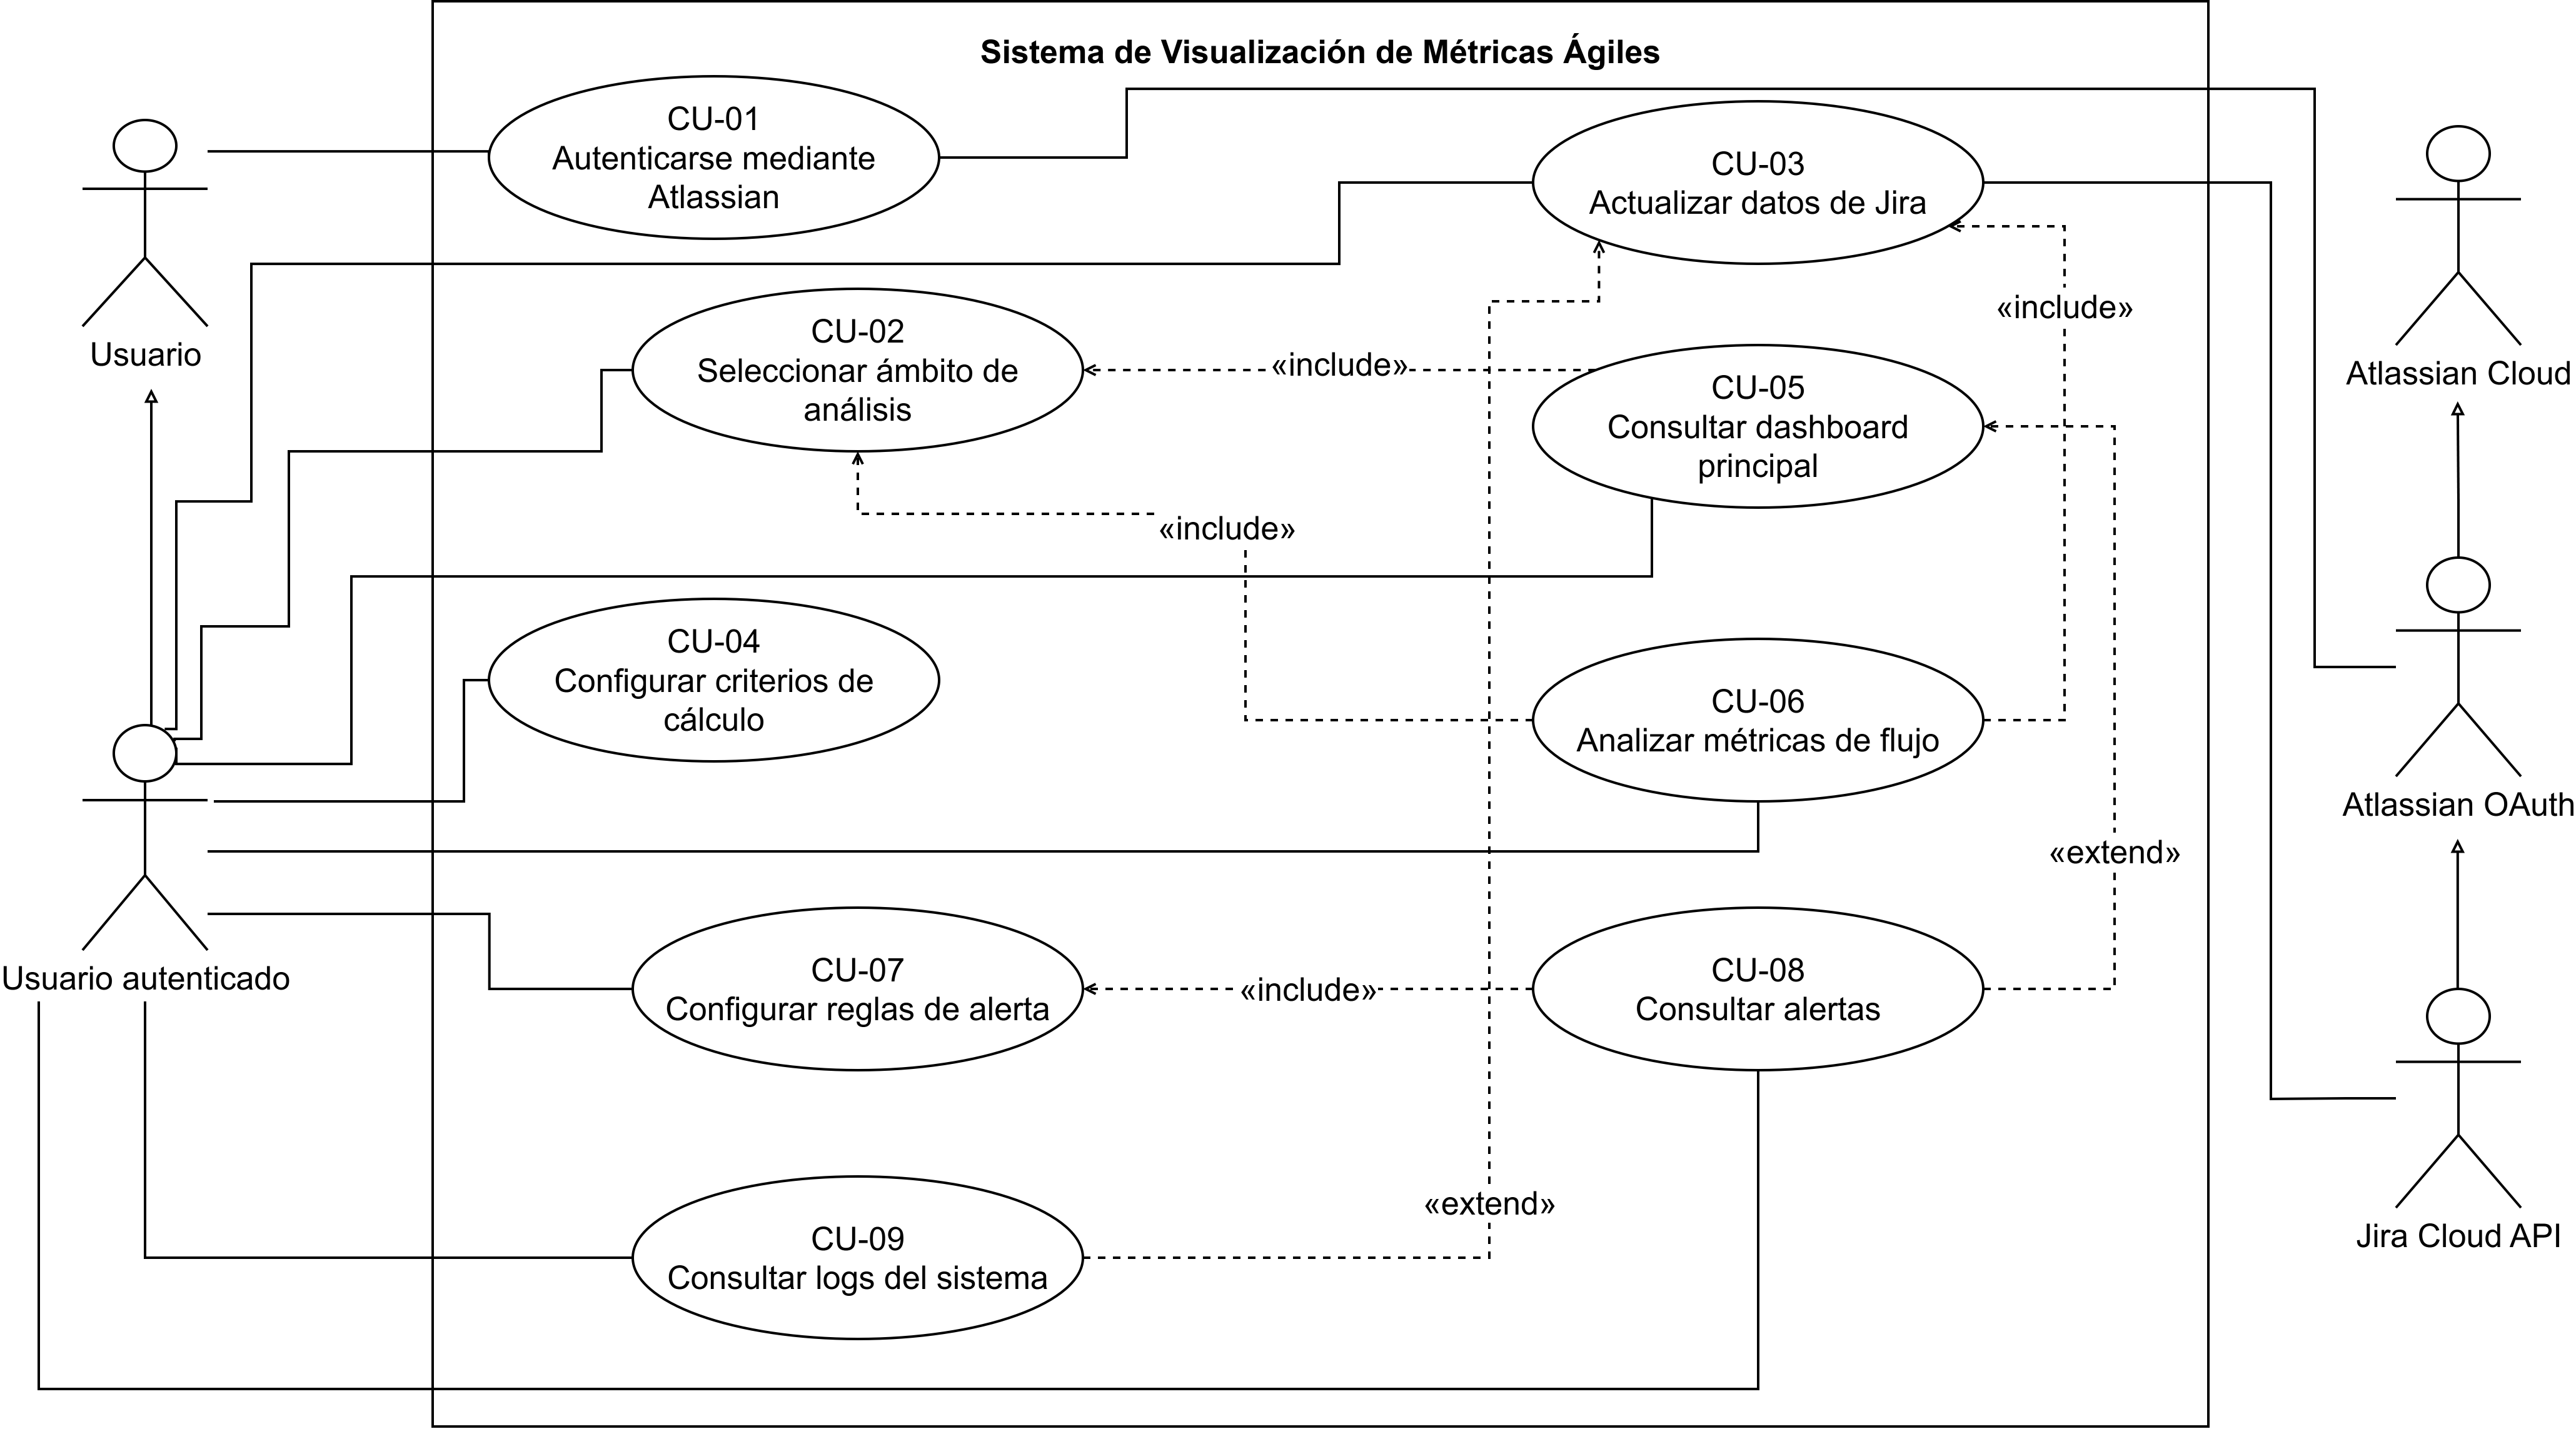
\includegraphics[width=\textwidth]{diagrams/casos-uso.png}
    \caption{Diagrama de casos de uso del sistema}
    \label{fig:casos-uso}
\end{figure}

Para facilitar su interpretación, se resumen a continuación los elementos principales del diagrama:

\begin{itemize}
    \item \textbf{Frontera del sistema}: el rectángulo delimita las funcionalidades que pertenecen al sistema de visualización de métricas ágiles.
    \item \textbf{Actores}: representan usuarios o sistemas externos que interactúan con el sistema.
    \item \textbf{Casos de uso}: las elipses identifican funcionalidades observables por los actores.
    \item \textbf{Generalización}: la flecha con triángulo hueco indica especialización entre actores.
    \item \textbf{Inclusión}: la relación \textit{include} indica que un caso de uso necesita ejecutar otro como parte de su comportamiento.
    \item \textbf{Extensión}: la relación \textit{extend} indica comportamiento opcional o condicionado que amplía otro caso de uso.
\end{itemize}

Los actores y sus relaciones principales son:

\begin{itemize}
    \item \textbf{Usuario}: actor general que puede iniciar el acceso al sistema mediante Atlassian.
    \item \textbf{Usuario autenticado}: especialización de \textit{Usuario}; puede seleccionar el ámbito de análisis, actualizar datos, consultar dashboards, analizar métricas, configurar reglas de alerta, consultar alertas y revisar logs.
    \item \textbf{Atlassian Cloud}: actor externo general que agrupa los servicios de Atlassian utilizados por el sistema.
    \item \textbf{Atlassian OAuth}: especialización de \textit{Atlassian Cloud}; participa en la autenticación mediante Atlassian.
    \item \textbf{Jira Cloud API}: especialización de \textit{Atlassian Cloud}; proporciona los datos de Jira necesarios para sincronización y cálculo de métricas.
\end{itemize}

Las relaciones entre casos de uso se interpretan de la siguiente forma:

\begin{itemize}
    \item \textbf{CU-05 incluye CU-02}: para consultar el dashboard principal es necesario seleccionar previamente el ámbito de análisis.
    \item \textbf{CU-06 incluye CU-02}: el análisis de métricas de flujo también depende del ámbito de análisis seleccionado.
    \item \textbf{CU-06 incluye CU-03}: para analizar métricas de flujo se requieren datos actualizados o previamente sincronizados desde Jira.
    \item \textbf{CU-08 incluye CU-07}: la consulta de alertas parte de reglas de alerta configuradas.
    \item \textbf{CU-08 extiende CU-05}: las alertas pueden complementar la consulta del dashboard cuando existan avisos relevantes.
    \item \textbf{CU-09 extiende CU-03}: los logs pueden consultarse como apoyo al diagnóstico de procesos de actualización, errores o eventos relevantes.
\end{itemize}

\clearpage
\section{Trazabilidad entre requisitos y casos de uso}

La trazabilidad permite comprobar que los casos de uso identificados cubren los requisitos funcionales principales. En esta fase inicial se plantea una matriz preliminar, que podrá ajustarse cuando se definan con mayor detalle los casos de uso y los diagramas asociados.

{\renewcommand{\arraystretch}{1.25}\scriptsize
\setlength{\tabcolsep}{3.2pt}
\begin{longtable}{|p{1.35cm}|c|c|c|c|c|c|c|c|c|}
\caption{Matriz de trazabilidad entre requisitos funcionales y casos de uso}\label{tab:trazabilidad-rf-cu}\\
\hline
\textbf{Req.} & \textbf{CU-01} & \textbf{CU-02} & \textbf{CU-03} & \textbf{CU-04} & \textbf{CU-05} & \textbf{CU-06} & \textbf{CU-07} & \textbf{CU-08} & \textbf{CU-09} \\
\hline
\endfirsthead
\hline
\textbf{Req.} & \textbf{CU-01} & \textbf{CU-02} & \textbf{CU-03} & \textbf{CU-04} & \textbf{CU-05} & \textbf{CU-06} & \textbf{CU-07} & \textbf{CU-08} & \textbf{CU-09} \\
\hline
\endhead
RF-01 &  &  & X &  &  &  &  &  &  \\\hline
RF-02 &  & X &  &  &  &  &  &  &  \\\hline
RF-03 &  &  & X &  &  &  &  &  &  \\\hline
RF-04 &  &  & X &  &  &  &  &  &  \\\hline
RF-05 &  &  & X &  &  &  &  &  &  \\\hline
RF-06 &  &  & X &  &  &  &  &  &  \\\hline
RF-07 &  & X &  & X &  &  &  &  &  \\\hline
RF-08 &  & X &  & X &  &  &  &  &  \\\hline
RF-09 &  &  &  &  & X & X &  &  &  \\\hline
RF-10 &  &  &  &  &  & X &  &  &  \\\hline
RF-11 &  &  & X &  &  &  &  &  &  \\\hline
RF-12 &  &  &  &  &  & X &  &  &  \\\hline
RF-13 &  &  &  &  &  & X &  &  &  \\\hline
RF-14 &  &  &  &  &  & X &  &  &  \\\hline
RF-15 &  &  &  &  &  & X &  &  &  \\\hline
RF-16 &  &  &  &  &  & X &  &  &  \\\hline
RF-17 &  &  &  &  &  & X &  &  &  \\\hline
RF-18 &  &  &  & X &  &  &  &  &  \\\hline
RF-19 &  &  &  &  & X &  &  &  &  \\\hline
RF-20 &  & X &  &  & X &  &  &  &  \\\hline
RF-21 &  &  &  &  & X &  &  &  &  \\\hline
RF-22 &  &  &  &  & X &  &  &  &  \\\hline
RF-23 &  &  &  &  & X &  &  &  &  \\\hline
RF-24 &  &  &  &  &  &  & X &  &  \\\hline
RF-25 &  &  &  &  &  &  &  & X &  \\\hline
RF-26 &  &  &  &  &  &  &  & X &  \\\hline
RF-27 &  &  &  &  &  &  &  &  & X \\\hline
RF-28 &  &  &  &  &  &  &  &  & X \\\hline
RF-29 & X &  &  &  &  &  &  &  &  \\\hline
RF-30 & X &  &  &  &  &  &  &  &  \\\hline
RF-31 & X &  &  &  &  &  &  &  &  \\\hline
\end{longtable}
\vspace{0.45em}
}

La matriz anterior no sustituye a la descripción detallada de los casos de uso. Su función es validar de forma visual que los requisitos funcionales quedan cubiertos por, al menos, un caso de uso identificado.
\clearpage
\section{Descripción detallada de los casos de uso}

Una vez identificados los casos de uso principales y validada su relación con los requisitos funcionales, se describen de forma detallada. Cada ficha recoge el actor principal, los actores secundarios, las precondiciones, el flujo principal, los posibles flujos alternativos, las postcondiciones y los requisitos relacionados. Esta descripción permite concretar el comportamiento esperado del sistema desde el punto de vista del usuario.

\subsection{CU-01: Autenticarse mediante Atlassian}

{\renewcommand{\arraystretch}{1.25}\footnotesize
\begin{longtable}{p{3.2cm}p{10.2cm}}
\toprule
\textbf{Campo} & \textbf{Descripción} \\
\midrule
\textbf{Actor principal} & Usuario. \\
\textbf{Actores secundarios} & Atlassian. \\
\textbf{Descripción} & Permite al usuario acceder al sistema utilizando el mecanismo oficial de autenticación de Atlassian, evitando el registro local de usuarios y el uso de credenciales propias de la aplicación. \\
\textbf{Precondiciones} & El usuario dispone de una cuenta válida de Atlassian. El servicio de autenticación de Atlassian está disponible. \\
\textbf{Flujo principal} & \begin{minipage}[t]{10.2cm}\begin{enumerate}[noitemsep,leftmargin=*]
    \item El usuario accede a la aplicación.
    \item El sistema muestra la opción de autenticación mediante Atlassian.
    \item El usuario selecciona iniciar sesión.
    \item El sistema redirige al usuario al mecanismo de autenticación de Atlassian.
    \item El usuario introduce sus credenciales en Atlassian y autoriza el acceso.
    \item Atlassian valida la autenticación y devuelve la respuesta al sistema.
    \item El sistema crea una sesión autenticada.
    \item El sistema muestra la pantalla principal de la aplicación.
\end{enumerate}\end{minipage} \\
\textbf{Flujos alternativos} & \begin{minipage}[t]{10.2cm}\begin{itemize}[noitemsep,leftmargin=*]
    \item El servicio de Atlassian no está disponible: el sistema informa de que no se puede completar la autenticación y el usuario permanece sin sesión iniciada.
    \item El usuario cancela el proceso de autenticación: el sistema vuelve a la pantalla inicial y no crea una sesión.
    \item La autenticación no es válida: el sistema informa de que no se ha podido iniciar sesión.
\end{itemize}\end{minipage} \\
\textbf{Postcondiciones} & El usuario queda autenticado en el sistema y puede acceder a las funcionalidades protegidas. \\
\textbf{Requisitos} & RF-29, RF-30, RF-31. \\
\bottomrule
\end{longtable}
\vspace{0.45em}
}

\clearpage
\subsection{CU-02: Seleccionar ámbito de análisis}

{\renewcommand{\arraystretch}{1.25}\footnotesize
\begin{longtable}{p{3.2cm}p{10.2cm}}
\toprule
\textbf{Campo} & \textbf{Descripción} \\
\midrule
\textbf{Actor principal} & Usuario autenticado. \\
\textbf{Actores secundarios} & Jira Cloud. \\
\textbf{Descripción} & Permite seleccionar el ámbito de datos sobre el que se desea trabajar, incluyendo proyecto, tablero, sprint, rango temporal, etiquetas, tipo de incidencia u otros criterios disponibles en Jira que se incorporen al sistema. \\
\textbf{Precondiciones} & El usuario ha iniciado sesión. El sistema dispone de conexión con Jira Cloud. Existen proyectos, tableros o datos disponibles para el usuario autenticado. \\
\textbf{Flujo principal} & \begin{minipage}[t]{10.2cm}\begin{enumerate}[noitemsep,leftmargin=*]
    \item El usuario accede a la sección de selección de ámbito.
    \item El sistema consulta los proyectos, tableros u opciones disponibles en Jira.
    \item El sistema muestra los criterios de selección disponibles.
    \item El usuario selecciona el proyecto, tablero, sprint, rango temporal u otros filtros.
    \item El sistema valida la selección realizada.
    \item El sistema guarda el ámbito de análisis seleccionado.
    \item El sistema actualiza las vistas o prepara la actualización de datos según el ámbito definido.
\end{enumerate}\end{minipage} \\
\textbf{Flujos alternativos} & \begin{minipage}[t]{10.2cm}\begin{itemize}[noitemsep,leftmargin=*]
    \item Jira Cloud no está disponible: el sistema informa de que no se pueden recuperar los datos y mantiene la selección anterior si existe.
    \item No existen proyectos o tableros disponibles: el sistema informa de que no se han encontrado ámbitos de análisis.
    \item La selección no es válida: el sistema informa del error y permite modificar los criterios seleccionados.
\end{itemize}\end{minipage} \\
\textbf{Postcondiciones} & El sistema dispone de un ámbito de análisis válido para actualizar datos, calcular métricas o filtrar visualizaciones. \\
\textbf{Requisitos} & RF-02, RF-07, RF-08, RF-20. \\
\bottomrule
\end{longtable}
\vspace{0.45em}
}

\clearpage
\subsection{CU-03: Actualizar datos de Jira}

{\renewcommand{\arraystretch}{1.25}\footnotesize
\begin{longtable}{p{3.2cm}p{10.2cm}}
\toprule
\textbf{Campo} & \textbf{Descripción} \\
\midrule
\textbf{Actor principal} & Usuario autenticado. \\
\textbf{Actores secundarios} & Jira Cloud. \\
\textbf{Descripción} & Permite actualizar los datos procedentes de Jira Cloud de forma controlada, reutilizando la información almacenada cuando siga siendo válida y evitando sincronizaciones completas innecesarias. \\
\textbf{Precondiciones} & El usuario ha iniciado sesión. Existe un ámbito de análisis seleccionado. La conexión con Jira Cloud está disponible cuando sea necesario consultar datos remotos. \\
\textbf{Flujo principal} & \begin{minipage}[t]{10.2cm}\begin{enumerate}[noitemsep,leftmargin=*]
    \item El usuario accede a un ámbito de análisis o solicita una actualización bajo demanda.
    \item El sistema comprueba la fecha de última actualización y el ámbito seleccionado.
    \item Si la información almacenada sigue siendo válida, el sistema reutiliza los datos disponibles.
    \item Si la información está desactualizada, el sistema consulta Jira Cloud API.
    \item El sistema importa o actualiza únicamente los datos necesarios cuando sea posible.
    \item El sistema registra la fecha y hora de actualización.
    \item El sistema detecta posibles datos incompletos o inconsistentes.
    \item El sistema recalcula las métricas afectadas.
    \item El sistema informa del estado de la actualización.
\end{enumerate}\end{minipage} \\
\textbf{Flujos alternativos} & \begin{minipage}[t]{10.2cm}\begin{itemize}[noitemsep,leftmargin=*]
    \item Jira Cloud no está disponible: el sistema informa del error, registra el evento y utiliza datos almacenados si existen.
    \item La API devuelve datos incompletos: el sistema registra la incidencia detectada y continúa con los datos válidos cuando sea posible.
    \item Se produce un error durante el cálculo de métricas: el sistema registra el error e informa de que la actualización se completó parcialmente.
\end{itemize}\end{minipage} \\
\textbf{Postcondiciones} & Los datos quedan actualizados o se reutilizan los datos almacenados válidos. Las métricas afectadas se recalculan cuando procede. \\
\textbf{Requisitos} & RF-01, RF-03, RF-04, RF-05, RF-06, RF-11. \\
\bottomrule
\end{longtable}
\vspace{0.45em}
}


\clearpage
\subsection{CU-04: Configurar criterios de cálculo de métricas}

{\renewcommand{\arraystretch}{1.25}\footnotesize
\begin{longtable}{p{3.2cm}p{10.2cm}}
\toprule
\textbf{Campo} & \textbf{Descripción} \\
\midrule
\textbf{Actor principal} & Usuario autenticado. \\
\textbf{Actores secundarios} & Ninguno. \\
\textbf{Descripción} & Permite definir cómo debe interpretar el sistema los datos procedentes de Jira para calcular métricas, incluyendo estados de inicio y fin, campo de esfuerzo, rango temporal, percentiles y criterios de agrupación. \\
\textbf{Precondiciones} & El usuario ha iniciado sesión. Existe un ámbito de análisis disponible. El sistema dispone de estados, campos o datos configurables. \\
\textbf{Flujo principal} & \begin{minipage}[t]{10.2cm}\begin{enumerate}[noitemsep,leftmargin=*]
    \item El usuario accede a la sección de configuración de criterios de cálculo.
    \item El sistema muestra los parámetros configurables según los datos disponibles.
    \item El usuario selecciona los estados que representan el inicio y el fin del trabajo efectivo.
    \item El usuario selecciona el campo de esfuerzo y otros criterios de análisis cuando proceda.
    \item El usuario ajusta percentiles, rango temporal o criterios de agrupación disponibles.
    \item El sistema valida la configuración introducida.
    \item El sistema guarda la configuración.
    \item El sistema aplica la configuración a los cálculos posteriores.
\end{enumerate}\end{minipage} \\
\textbf{Flujos alternativos} & \begin{minipage}[t]{10.2cm}\begin{itemize}[noitemsep,leftmargin=*]
    \item El usuario no selecciona estados válidos: el sistema informa del problema y solicita corregir la configuración.
    \item Algún parámetro es incompatible con los datos disponibles: el sistema informa del campo afectado y permite modificarlo.
    \item El usuario cancela la configuración: el sistema mantiene la configuración anterior.
\end{itemize}\end{minipage} \\
\textbf{Postcondiciones} & La configuración queda guardada y se utiliza para calcular las métricas del sistema. \\
\textbf{Requisitos} & RF-07, RF-08, RF-18. \\
\bottomrule
\end{longtable}
\vspace{0.45em}
}

\clearpage
\subsection{CU-05: Consultar dashboard principal}

{\renewcommand{\arraystretch}{1.25}\footnotesize
\begin{longtable}{p{3.2cm}p{10.2cm}}
\toprule
\textbf{Campo} & \textbf{Descripción} \\
\midrule
\textbf{Actor principal} & Usuario autenticado. \\
\textbf{Actores secundarios} & Ninguno. \\
\textbf{Descripción} & Permite visualizar en un dashboard principal las métricas clave del sistema para un periodo y ámbito de análisis seleccionados. \\
\textbf{Precondiciones} & El usuario ha iniciado sesión. Existe un ámbito de análisis seleccionado. El sistema dispone de datos sincronizados, almacenados o de demostración. \\
\textbf{Flujo principal} & \begin{minipage}[t]{10.2cm}\begin{enumerate}[noitemsep,leftmargin=*]
    \item El usuario accede al dashboard principal.
    \item El sistema obtiene las métricas disponibles para el ámbito seleccionado.
    \item El sistema muestra las métricas clave mediante widgets o visualizaciones.
    \item El usuario modifica filtros o rango temporal si lo desea.
    \item El sistema actualiza el dashboard según los filtros aplicados.
    \item El usuario consulta la información mostrada.
\end{enumerate}\end{minipage} \\
\textbf{Flujos alternativos} & \begin{minipage}[t]{10.2cm}\begin{itemize}[noitemsep,leftmargin=*]
    \item No existen datos disponibles: el sistema informa de la situación y puede mostrar datos de demostración si existen.
    \item Los filtros no devuelven resultados: el sistema informa de que no hay información para los criterios seleccionados.
\end{itemize}\end{minipage} \\
\textbf{Postcondiciones} & El usuario visualiza el estado general del proyecto o equipo mediante las métricas disponibles. \\
\textbf{Requisitos} & RF-09, RF-19, RF-20, RF-21, RF-22, RF-23. \\
\bottomrule
\end{longtable}
\vspace{0.45em}
}

\clearpage
\subsection{CU-06: Analizar métricas de flujo}

{\renewcommand{\arraystretch}{1.25}\footnotesize
\begin{longtable}{p{3.2cm}p{10.2cm}}
\toprule
\textbf{Campo} & \textbf{Descripción} \\
\midrule
\textbf{Actor principal} & Usuario autenticado. \\
\textbf{Actores secundarios} & Ninguno. \\
\textbf{Descripción} & Permite consultar métricas de flujo y rendimiento del equipo, como Velocity, WIP, Lead Time, Cycle Time y otras métricas adicionales cuando existan datos suficientes. \\
\textbf{Precondiciones} & El usuario ha iniciado sesión. El sistema dispone de datos sincronizados o almacenados. Los criterios necesarios para el cálculo de métricas están configurados. \\
\textbf{Flujo principal} & \begin{minipage}[t]{10.2cm}\begin{enumerate}[noitemsep,leftmargin=*]
    \item El usuario accede a la vista de análisis de métricas.
    \item El sistema muestra las métricas disponibles para el ámbito seleccionado.
    \item El usuario selecciona una métrica o conjunto de métricas.
    \item El sistema muestra los valores calculados y su evolución cuando proceda.
    \item El usuario aplica filtros o cambia el periodo de análisis.
    \item El sistema recalcula o actualiza la visualización.
    \item El usuario interpreta los resultados mostrados.
\end{enumerate}\end{minipage} \\
\textbf{Flujos alternativos} & \begin{minipage}[t]{10.2cm}\begin{itemize}[noitemsep,leftmargin=*]
    \item No existen datos suficientes para una métrica: el sistema informa de que la métrica no puede calcularse e indica, cuando sea posible, qué datos faltan.
    \item Se produce un error en el cálculo: el sistema registra el error e informa al usuario.
\end{itemize}\end{minipage} \\
\textbf{Postcondiciones} & El usuario dispone de información analítica sobre el flujo de trabajo y las métricas seleccionadas. \\
\textbf{Requisitos} & RF-09, RF-10, RF-12, RF-13, RF-14, RF-15, RF-16, RF-17. \\
\bottomrule
\end{longtable}
\vspace{0.45em}
}

\clearpage
\subsection{CU-07: Configurar reglas de alerta}

{\renewcommand{\arraystretch}{1.25}\footnotesize
\begin{longtable}{p{3.2cm}p{10.2cm}}
\toprule
\textbf{Campo} & \textbf{Descripción} \\
\midrule
\textbf{Actor principal} & Usuario autenticado. \\
\textbf{Actores secundarios} & Ninguno. \\
\textbf{Descripción} & Permite definir reglas de alerta simples basadas en umbrales configurables sobre métricas calculadas, como WIP, Cycle Time, Lead Time o Velocity. \\
\textbf{Precondiciones} & El usuario ha iniciado sesión. El sistema dispone de métricas calculadas o configurables. El usuario conoce el umbral que desea establecer. \\
\textbf{Flujo principal} & \begin{minipage}[t]{10.2cm}\begin{enumerate}[noitemsep,leftmargin=*]
    \item El usuario accede a la sección de configuración de alertas.
    \item El sistema muestra las métricas disponibles para crear reglas.
    \item El usuario selecciona la métrica sobre la que quiere definir una alerta.
    \item El usuario introduce el umbral o condición simple.
    \item El usuario guarda la regla de alerta.
    \item El sistema valida la regla introducida.
    \item El sistema almacena la regla.
    \item El sistema evalúa la regla cuando se actualicen las métricas.
\end{enumerate}\end{minipage} \\
\textbf{Flujos alternativos} & \begin{minipage}[t]{10.2cm}\begin{itemize}[noitemsep,leftmargin=*]
    \item El usuario introduce un umbral no válido: el sistema informa del error y solicita corregir el valor.
    \item La regla no puede aplicarse a la métrica seleccionada: el sistema informa de la incompatibilidad y permite modificar la regla.
\end{itemize}\end{minipage} \\
\textbf{Postcondiciones} & La regla de alerta queda registrada y podrá activarse cuando se cumpla la condición definida. \\
\textbf{Requisitos} & RF-24. \\
\bottomrule
\end{longtable}
\vspace{0.45em}
}

\clearpage
\subsection{CU-08: Consultar alertas}

{\renewcommand{\arraystretch}{1.25}\footnotesize
\begin{longtable}{p{3.2cm}p{10.2cm}}
\toprule
\textbf{Campo} & \textbf{Descripción} \\
\midrule
\textbf{Actor principal} & Usuario autenticado. \\
\textbf{Actores secundarios} & Ninguno. \\
\textbf{Descripción} & Permite consultar alertas activas e históricas conservadas por el sistema, incluyendo su estado, momento de activación, métrica asociada y periodo de disponibilidad. \\
\textbf{Precondiciones} & El usuario ha iniciado sesión. Existen reglas de alerta configuradas. El sistema ha evaluado las métricas disponibles. \\
\textbf{Flujo principal} & \begin{minipage}[t]{10.2cm}\begin{enumerate}[noitemsep,leftmargin=*]
    \item El usuario accede a la sección de alertas.
    \item El sistema muestra las alertas activas e históricas conservadas.
    \item El usuario filtra las alertas por estado, métrica o periodo si lo desea.
    \item El sistema actualiza la lista de alertas según los filtros aplicados.
    \item El usuario consulta el detalle de una alerta.
\end{enumerate}\end{minipage} \\
\textbf{Flujos alternativos} & \begin{minipage}[t]{10.2cm}\begin{itemize}[noitemsep,leftmargin=*]
    \item No existen alertas registradas: el sistema informa de que no hay alertas disponibles.
    \item Los filtros no devuelven resultados: el sistema informa de que no existen alertas para los criterios seleccionados.
    \item La alerta histórica ha expirado según la política de retención: el sistema no la muestra en la consulta ordinaria.
\end{itemize}\end{minipage} \\
\textbf{Postcondiciones} & El usuario visualiza las alertas relevantes disponibles según los filtros aplicados y la política de retención definida. \\
\textbf{Requisitos} & RF-25, RF-26. \\
\bottomrule
\end{longtable}
\vspace{0.45em}
}

\clearpage
\subsection{CU-09: Consultar logs del sistema}

{\renewcommand{\arraystretch}{1.25}\footnotesize
\begin{longtable}{p{3.2cm}p{10.2cm}}
\toprule
\textbf{Campo} & \textbf{Descripción} \\
\midrule
\textbf{Actor principal} & Usuario autenticado. \\
\textbf{Actores secundarios} & Ninguno. \\
\textbf{Descripción} & Permite consultar eventos relevantes generados por el sistema, como actualizaciones de datos, errores de integración, errores de cálculo o eventos de autenticación asociados al uso de la aplicación. \\
\textbf{Precondiciones} & El usuario ha iniciado sesión. Existen eventos registrados por el sistema. \\
\textbf{Flujo principal} & \begin{minipage}[t]{10.2cm}\begin{enumerate}[noitemsep,leftmargin=*]
    \item El usuario accede a la sección de logs.
    \item El sistema muestra una lista de eventos registrados.
    \item El usuario aplica filtros básicos si lo considera necesario.
    \item El sistema actualiza la lista según los criterios seleccionados.
    \item El usuario consulta el detalle de un evento concreto.
\end{enumerate}\end{minipage} \\
\textbf{Flujos alternativos} & \begin{minipage}[t]{10.2cm}\begin{itemize}[noitemsep,leftmargin=*]
    \item No existen logs disponibles: el sistema informa de que no hay eventos registrados.
    \item No hay resultados para los filtros aplicados: el sistema muestra un mensaje indicando que no se han encontrado eventos.
    \item Algunos logs han expirado según la política de retención: el sistema no los muestra en la consulta ordinaria.
\end{itemize}\end{minipage} \\
\textbf{Postcondiciones} & El usuario visualiza los eventos relevantes disponibles según los filtros aplicados y la política de retención definida. \\
\textbf{Requisitos} & RF-27, RF-28. \\
\bottomrule
\end{longtable}
\vspace{0.45em}
}

\clearpage
\section{Diagramas de secuencia}

Los diagramas de secuencia complementan la descripción textual de los casos de uso mostrando el orden temporal de los mensajes intercambiados entre el usuario, la aplicación y los servicios externos. En esta memoria se incluyen únicamente los casos de uso más representativos, ya que son los que concentran la interacción con Atlassian, Jira Cloud API y la lógica principal del sistema.

\subsection{CU-01: Autenticarse mediante Atlassian}

Este diagrama de secuencia describe el comportamiento asociado al caso de uso CU-01, centrado en el inicio de sesión del usuario mediante el proveedor de autenticación de Atlassian.

\begin{figure}[htbp]
    \centering
    \makebox[\textwidth][c]{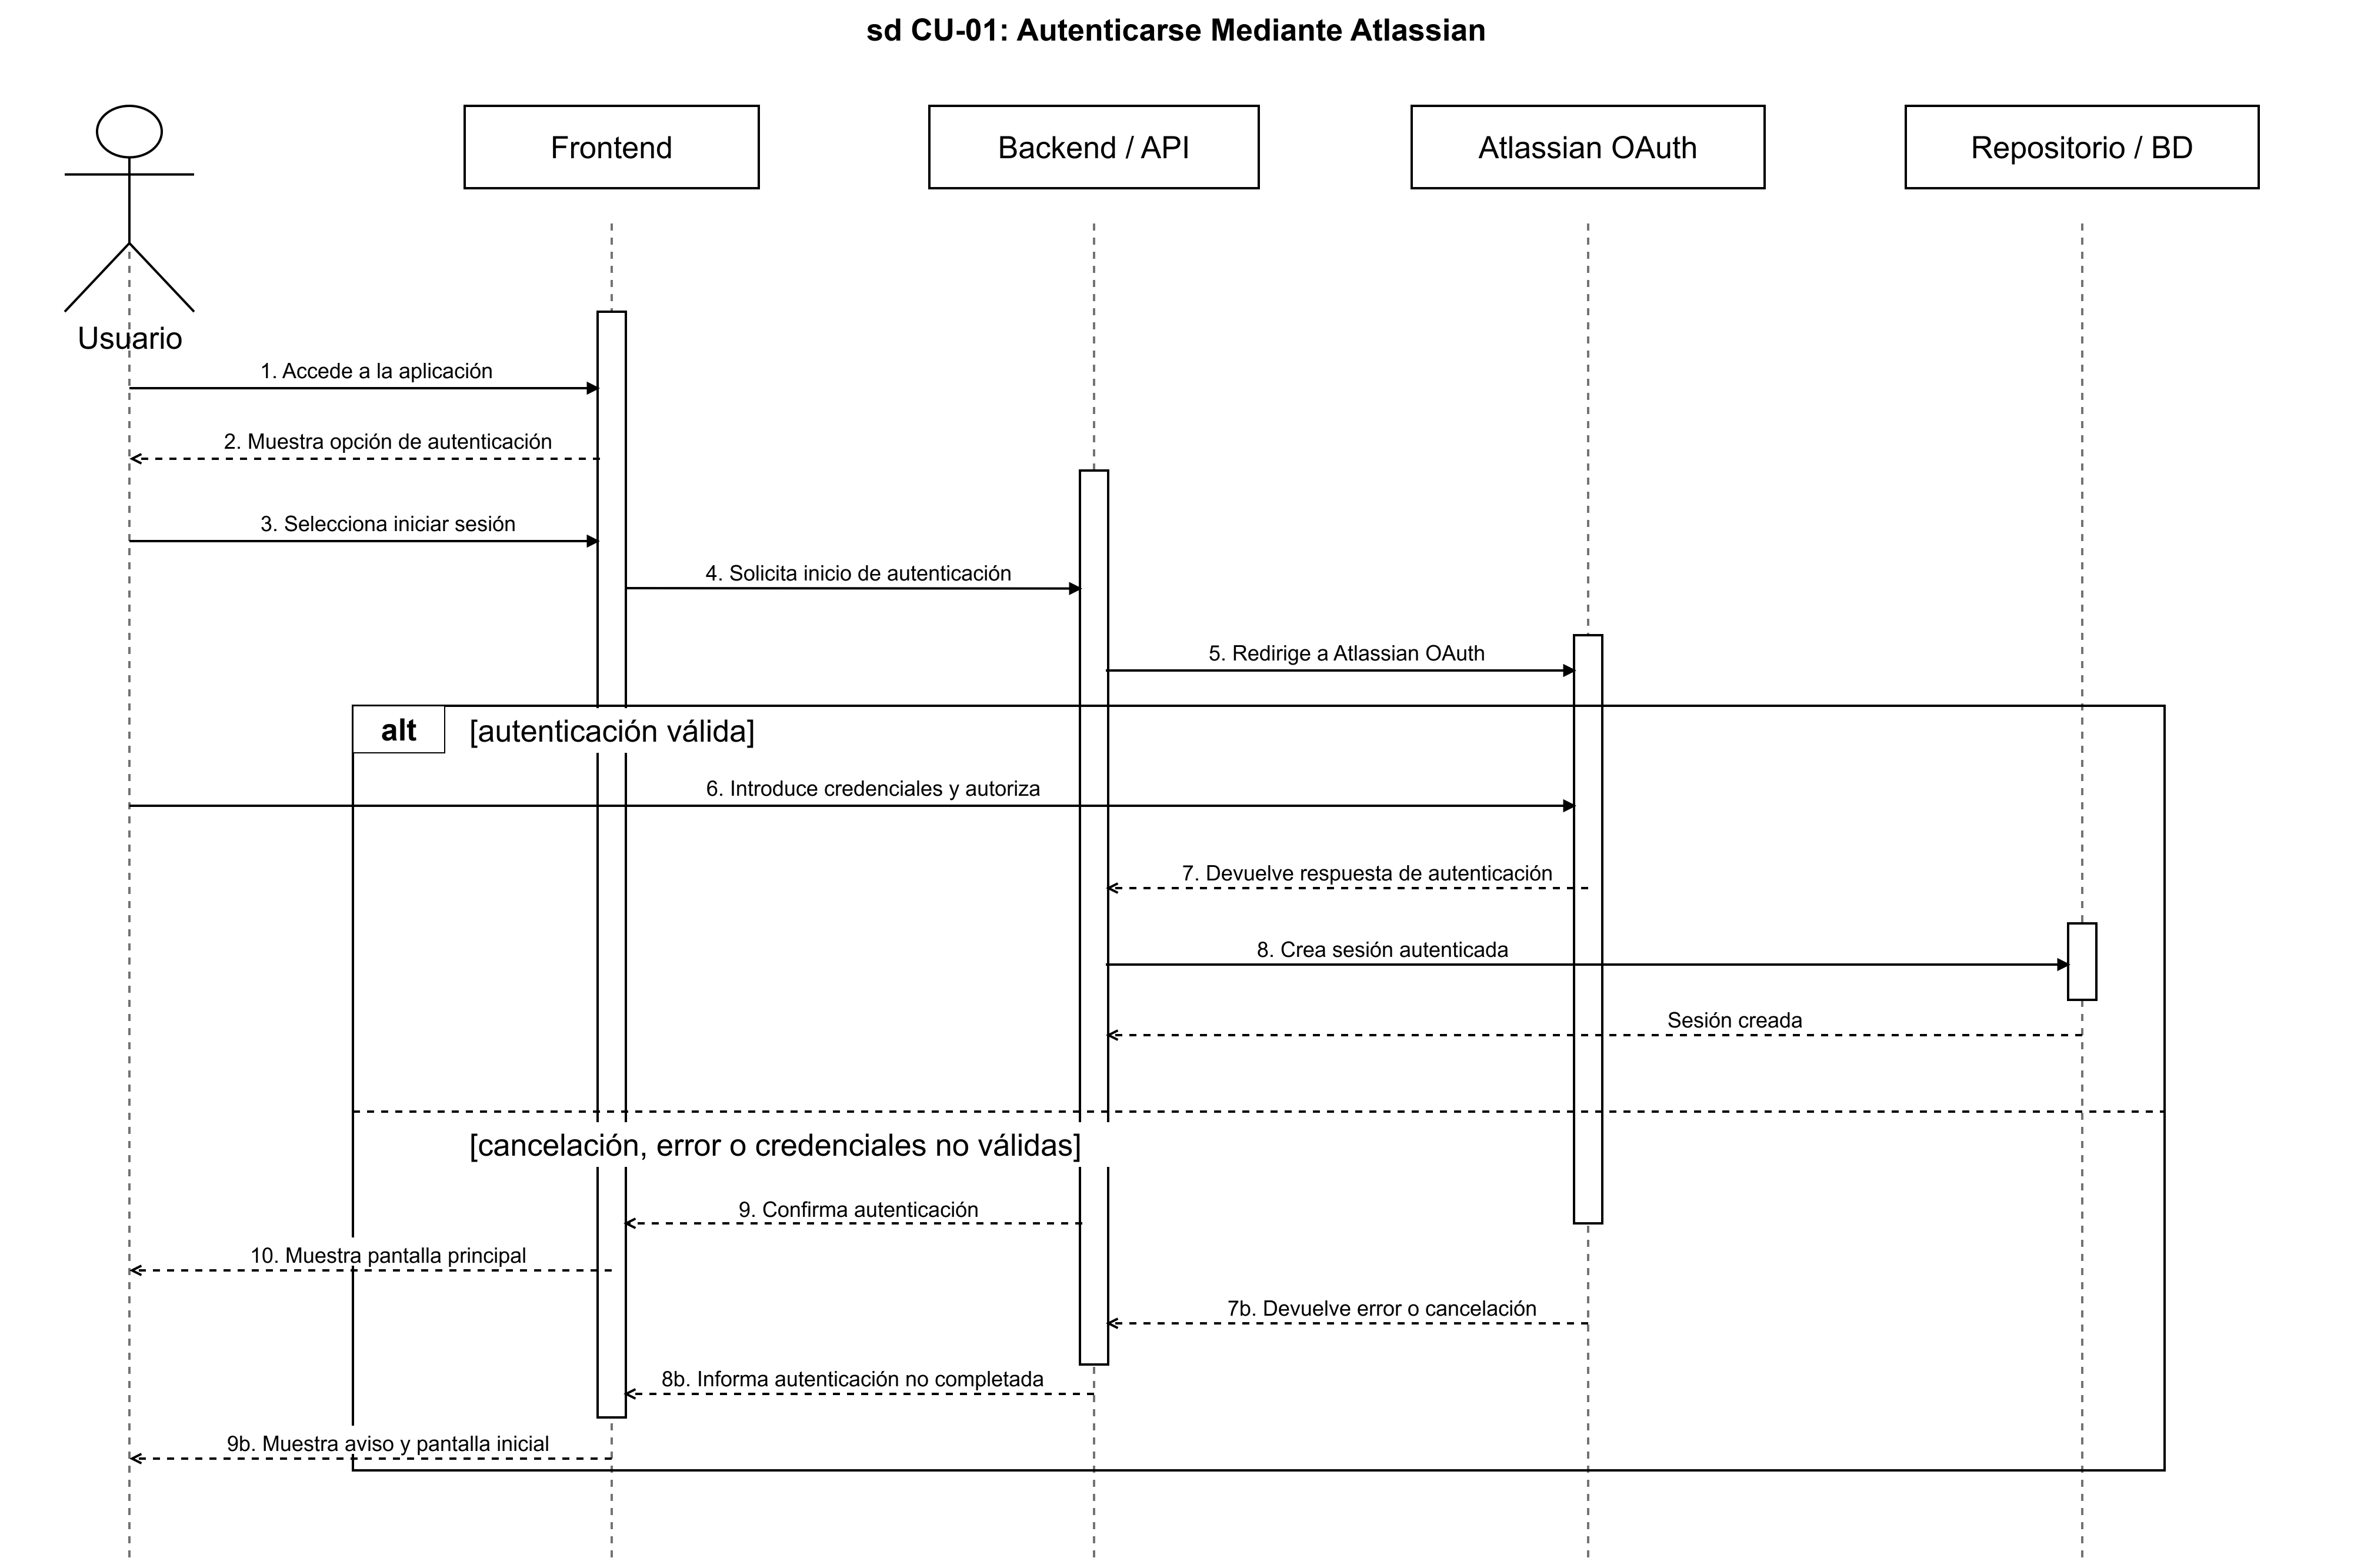
\includegraphics[width=1.08\textwidth]{diagrams/secuencia-cu01-autenticarse-atlassian.png}}
    \caption{Diagrama de secuencia del caso de uso CU-01}
    \label{fig:secuencia-cu01-autenticarse-atlassian}
\end{figure}

La Figura~\ref{fig:secuencia-cu01-autenticarse-atlassian} representa el proceso de autenticación mediante Atlassian. El usuario inicia sesión desde la aplicación, el sistema redirige la operación hacia Atlassian OAuth y, si la autenticación es válida, se crea una sesión autenticada. También se contempla el caso alternativo en el que el usuario cancela el proceso o Atlassian devuelve un error.

\subsection{CU-03: Actualizar datos de Jira}

Este diagrama de secuencia describe el comportamiento asociado al caso de uso CU-03, correspondiente a la actualización de la información procedente de Jira y al tratamiento posterior de los datos obtenidos.

\begin{figure}[htbp]
    \centering
    \makebox[\textwidth][c]{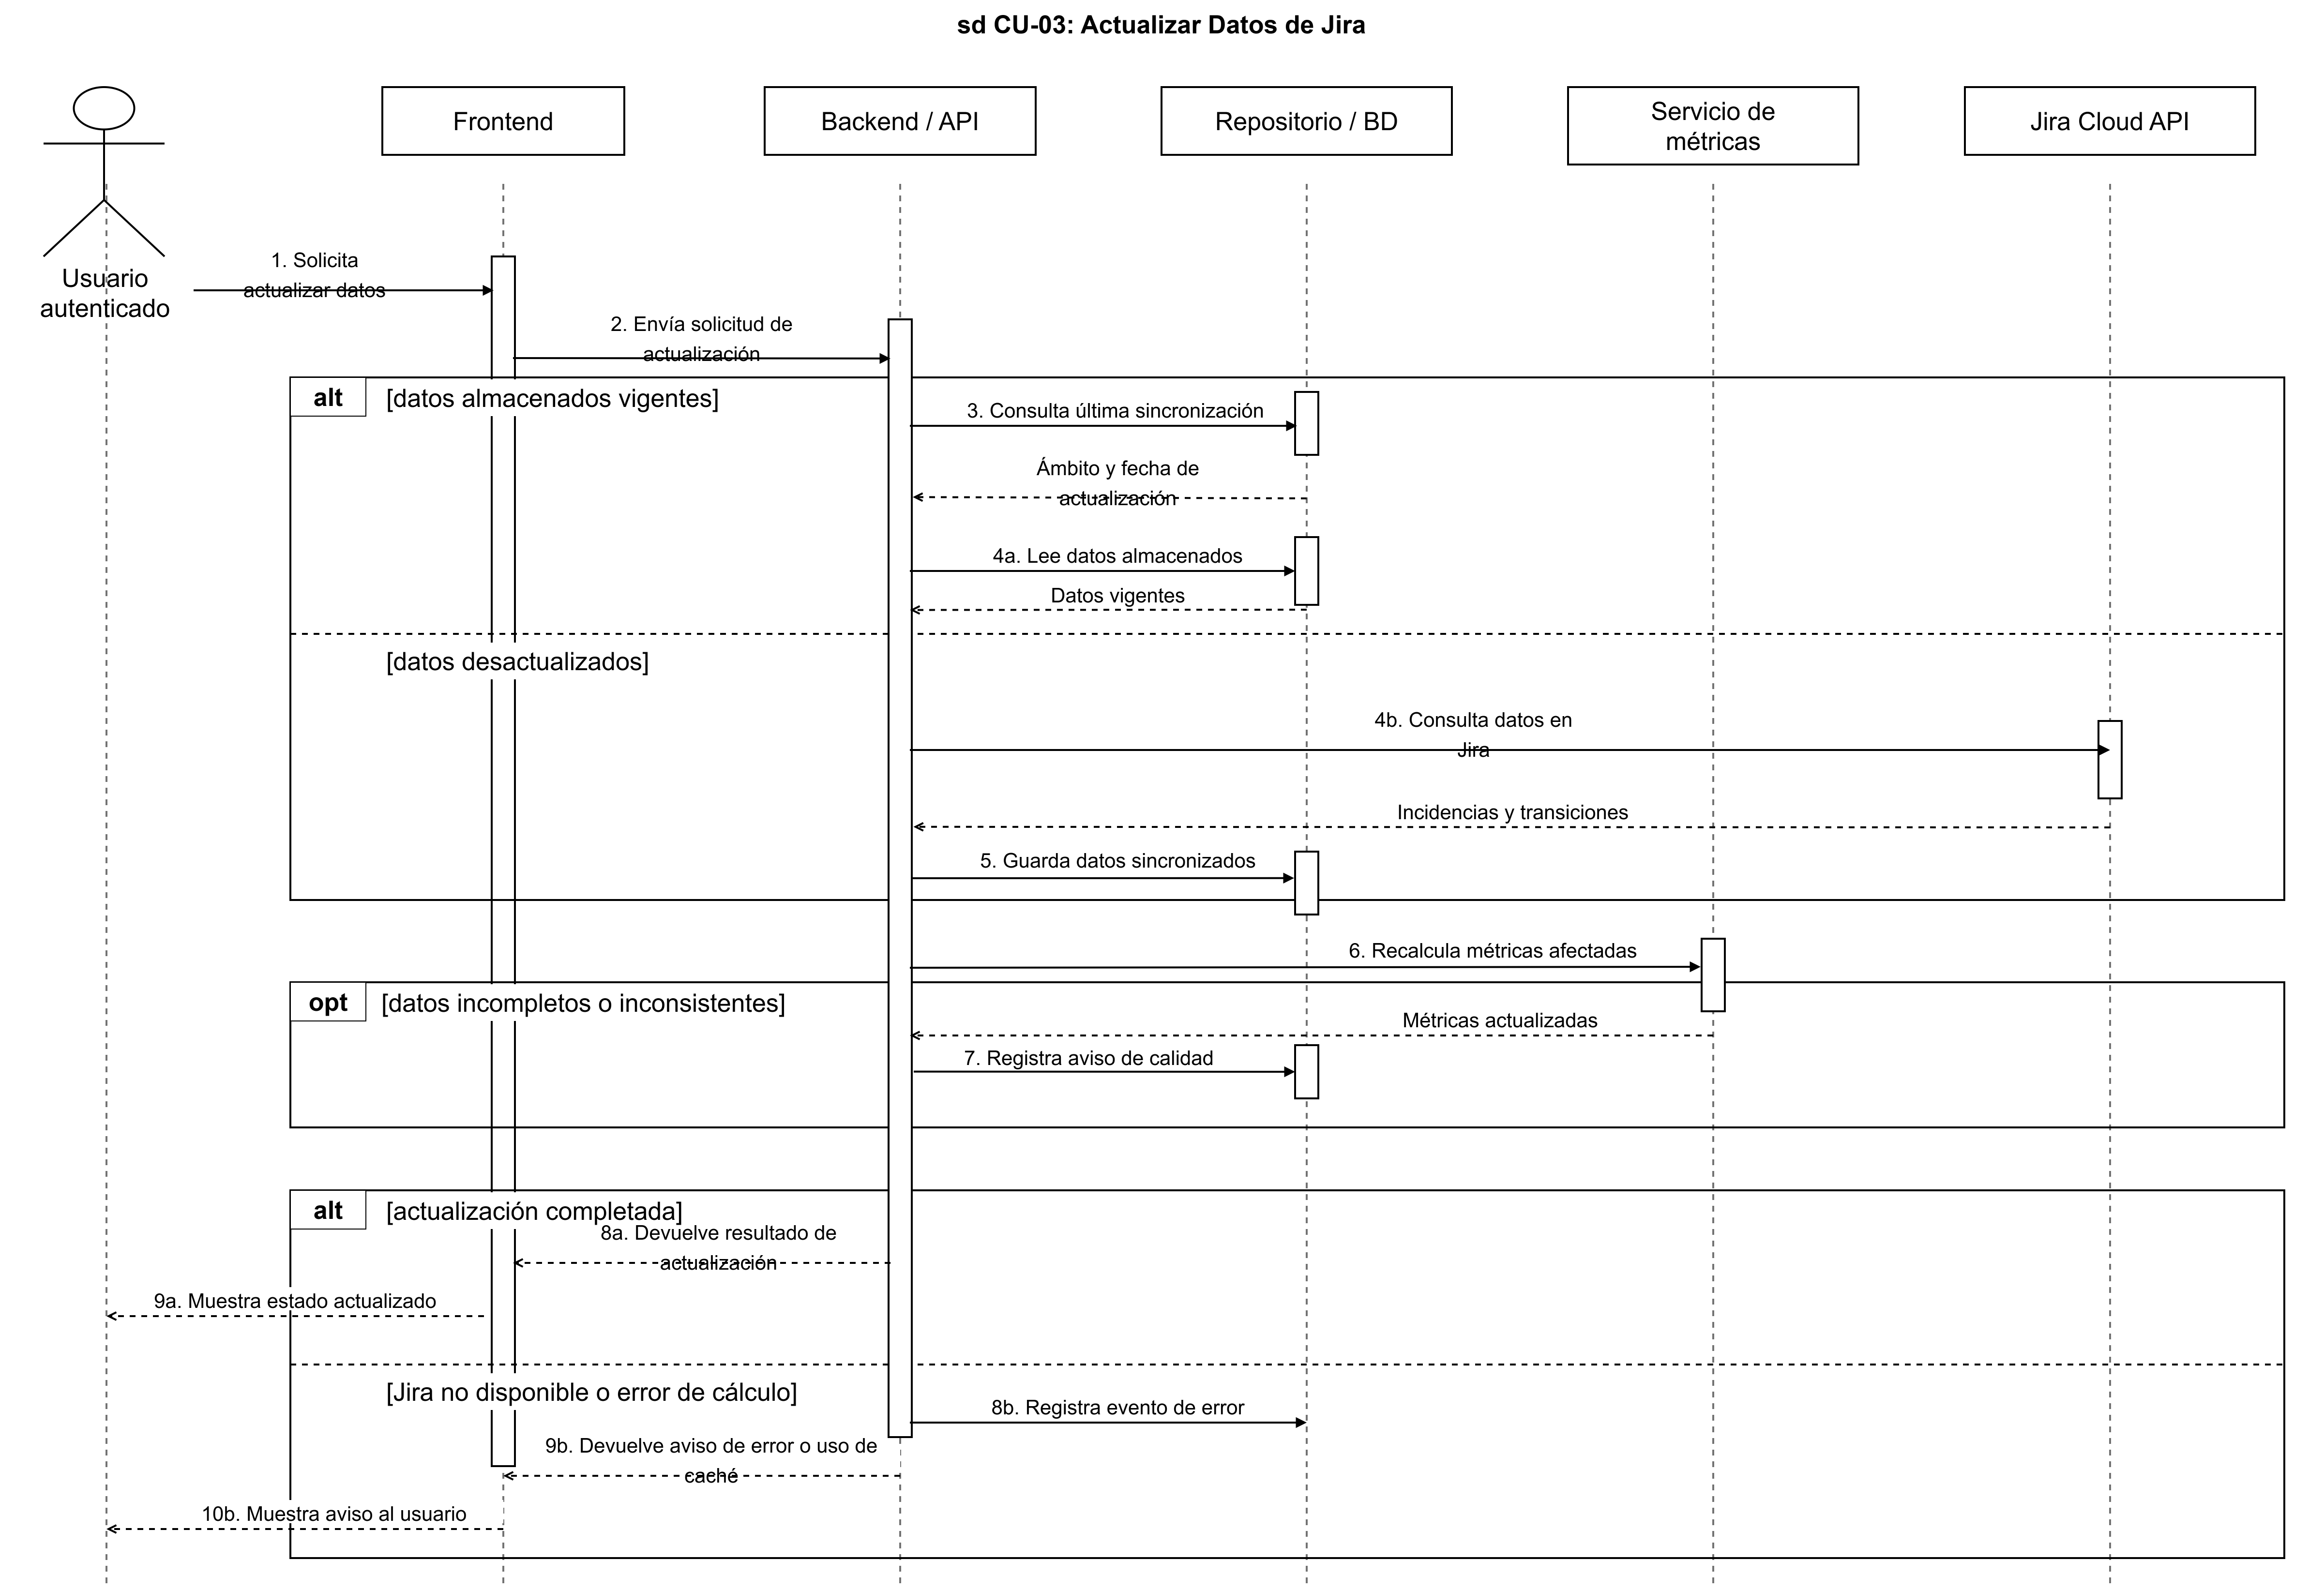
\includegraphics[width=1.08\textwidth]{diagrams/secuencia-cu03-actualizar-datos-jira.png}}
    \caption{Diagrama de secuencia del caso de uso CU-03}
    \label{fig:secuencia-cu03-actualizar-datos-jira}
\end{figure}

La Figura~\ref{fig:secuencia-cu03-actualizar-datos-jira} resume la actualización de datos desde Jira. El usuario autenticado solicita la actualización, el sistema comprueba si los datos almacenados siguen siendo válidos y, en caso contrario, consulta Jira Cloud API. A continuación, persiste la información obtenida, recalcula las métricas afectadas y comunica el resultado, contemplando también situaciones de error o datos incompletos.

\newpage

\subsection{CU-05: Consultar dashboard principal}

Este diagrama de secuencia describe el comportamiento asociado al caso de uso CU-05, centrado en la visualización del dashboard principal para un ámbito de análisis y unos filtros determinados.

\begin{figure}[htbp]
    \centering
    \makebox[\textwidth][c]{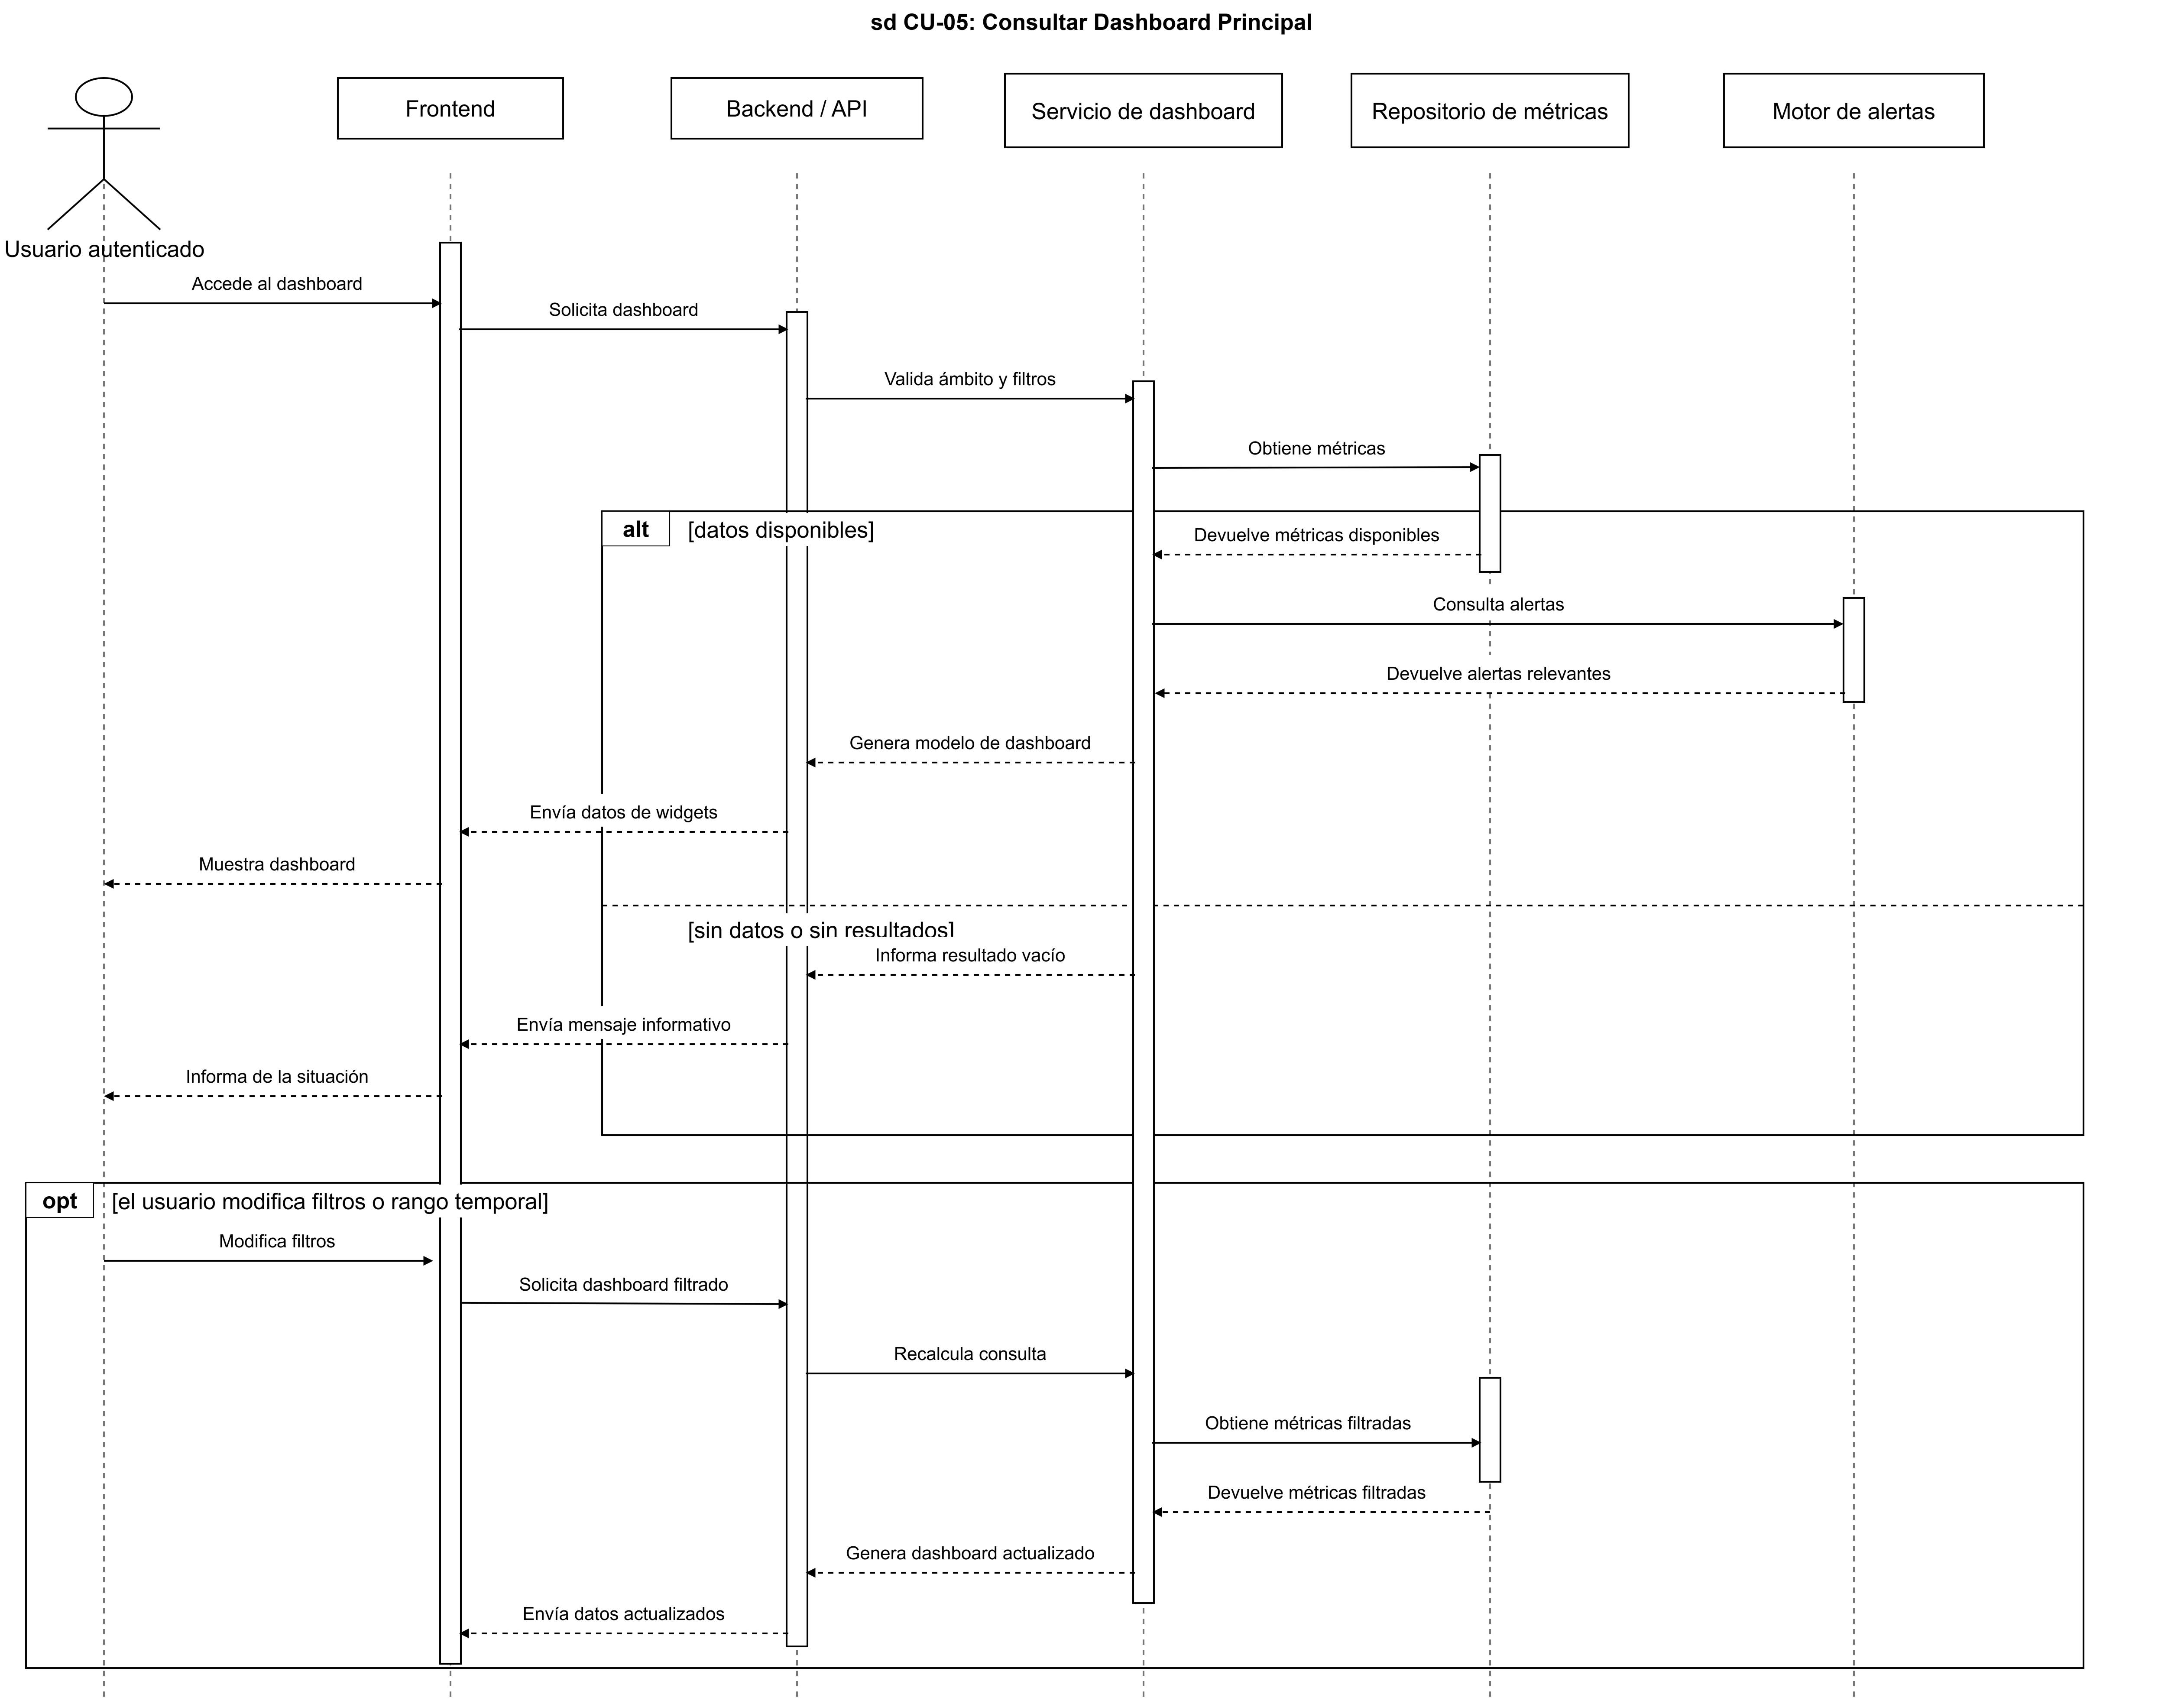
\includegraphics[width=1.08\textwidth]{diagrams/secuencia-cu05-consultar-dashboard-principal.png}}
    \caption{Diagrama de secuencia del caso de uso CU-05}
    \label{fig:secuencia-cu05-consultar-dashboard-principal}
\end{figure}

La Figura~\ref{fig:secuencia-cu05-consultar-dashboard-principal} muestra cómo el usuario autenticado accede al dashboard, el frontend solicita los datos al backend y el sistema valida el ámbito y los filtros antes de recuperar las métricas disponibles. El diagrama contempla la respuesta normal con los datos necesarios para construir los widgets, el caso alternativo en el que no existen datos o los filtros no devuelven resultados, y la actualización del dashboard cuando el usuario modifica los filtros o el rango temporal.

\subsection{CU-06: Analizar métricas de flujo}

Este diagrama de secuencia describe el comportamiento asociado al caso de uso CU-06, centrado en la consulta de métricas de flujo y rendimiento a partir de los datos sincronizados y los criterios de cálculo configurados.

\begin{figure}[htbp]
    \centering
    \makebox[\textwidth][c]{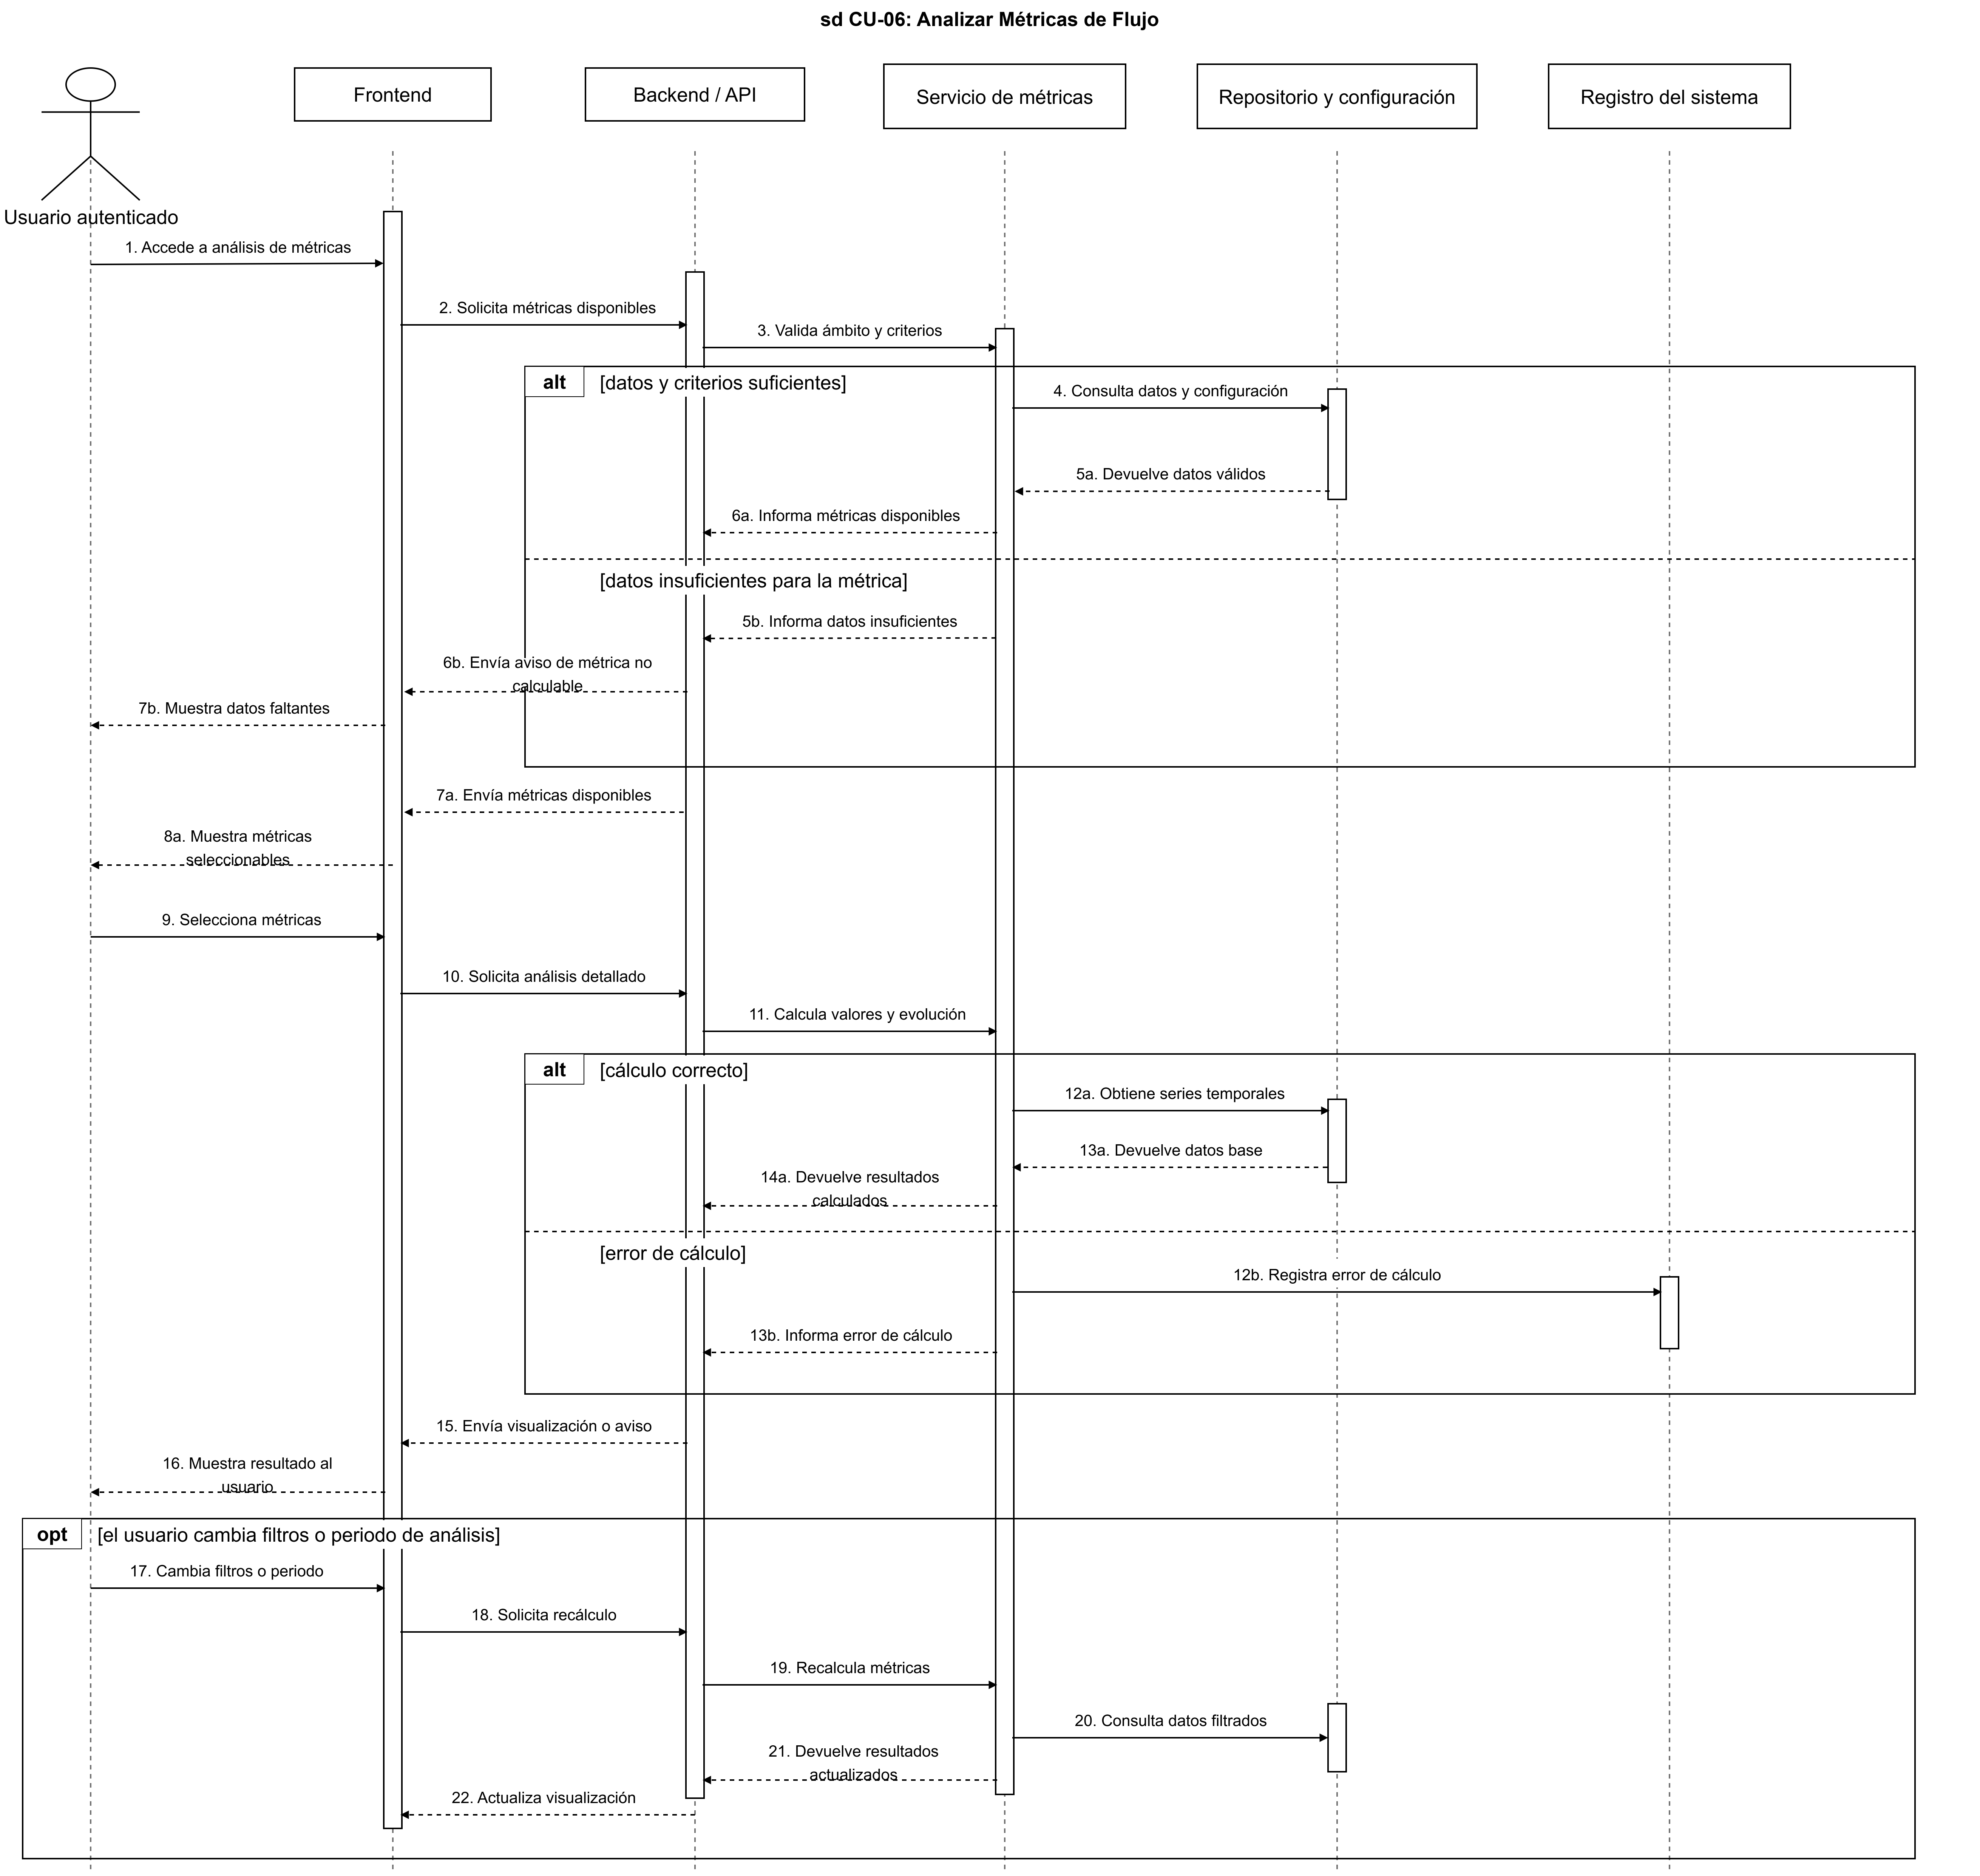
\includegraphics[width=1.08\textwidth]{diagrams/secuencia-cu06-analizar-metricas-flujo.png}}
    \caption{Diagrama de secuencia del caso de uso CU-06}
    \label{fig:secuencia-cu06-analizar-metricas-flujo}
\end{figure}

La Figura~\ref{fig:secuencia-cu06-analizar-metricas-flujo} muestra cómo el usuario autenticado accede a la vista de análisis, el sistema valida el ámbito seleccionado y recupera los datos y criterios necesarios para calcular las métricas disponibles. El diagrama contempla el flujo normal de selección y cálculo de métricas, el caso alternativo en el que no existen datos suficientes, el registro de errores de cálculo y la actualización de resultados cuando el usuario modifica filtros o el periodo de análisis.

\newpage

\subsection{CU-07: Configurar reglas de alerta}

Este diagrama de secuencia describe el comportamiento asociado al caso de uso CU-07, centrado en la creación de reglas de alerta a partir de métricas disponibles y condiciones simples definidas por el usuario.

\begin{figure}[htbp]
    \centering
    \makebox[\textwidth][c]{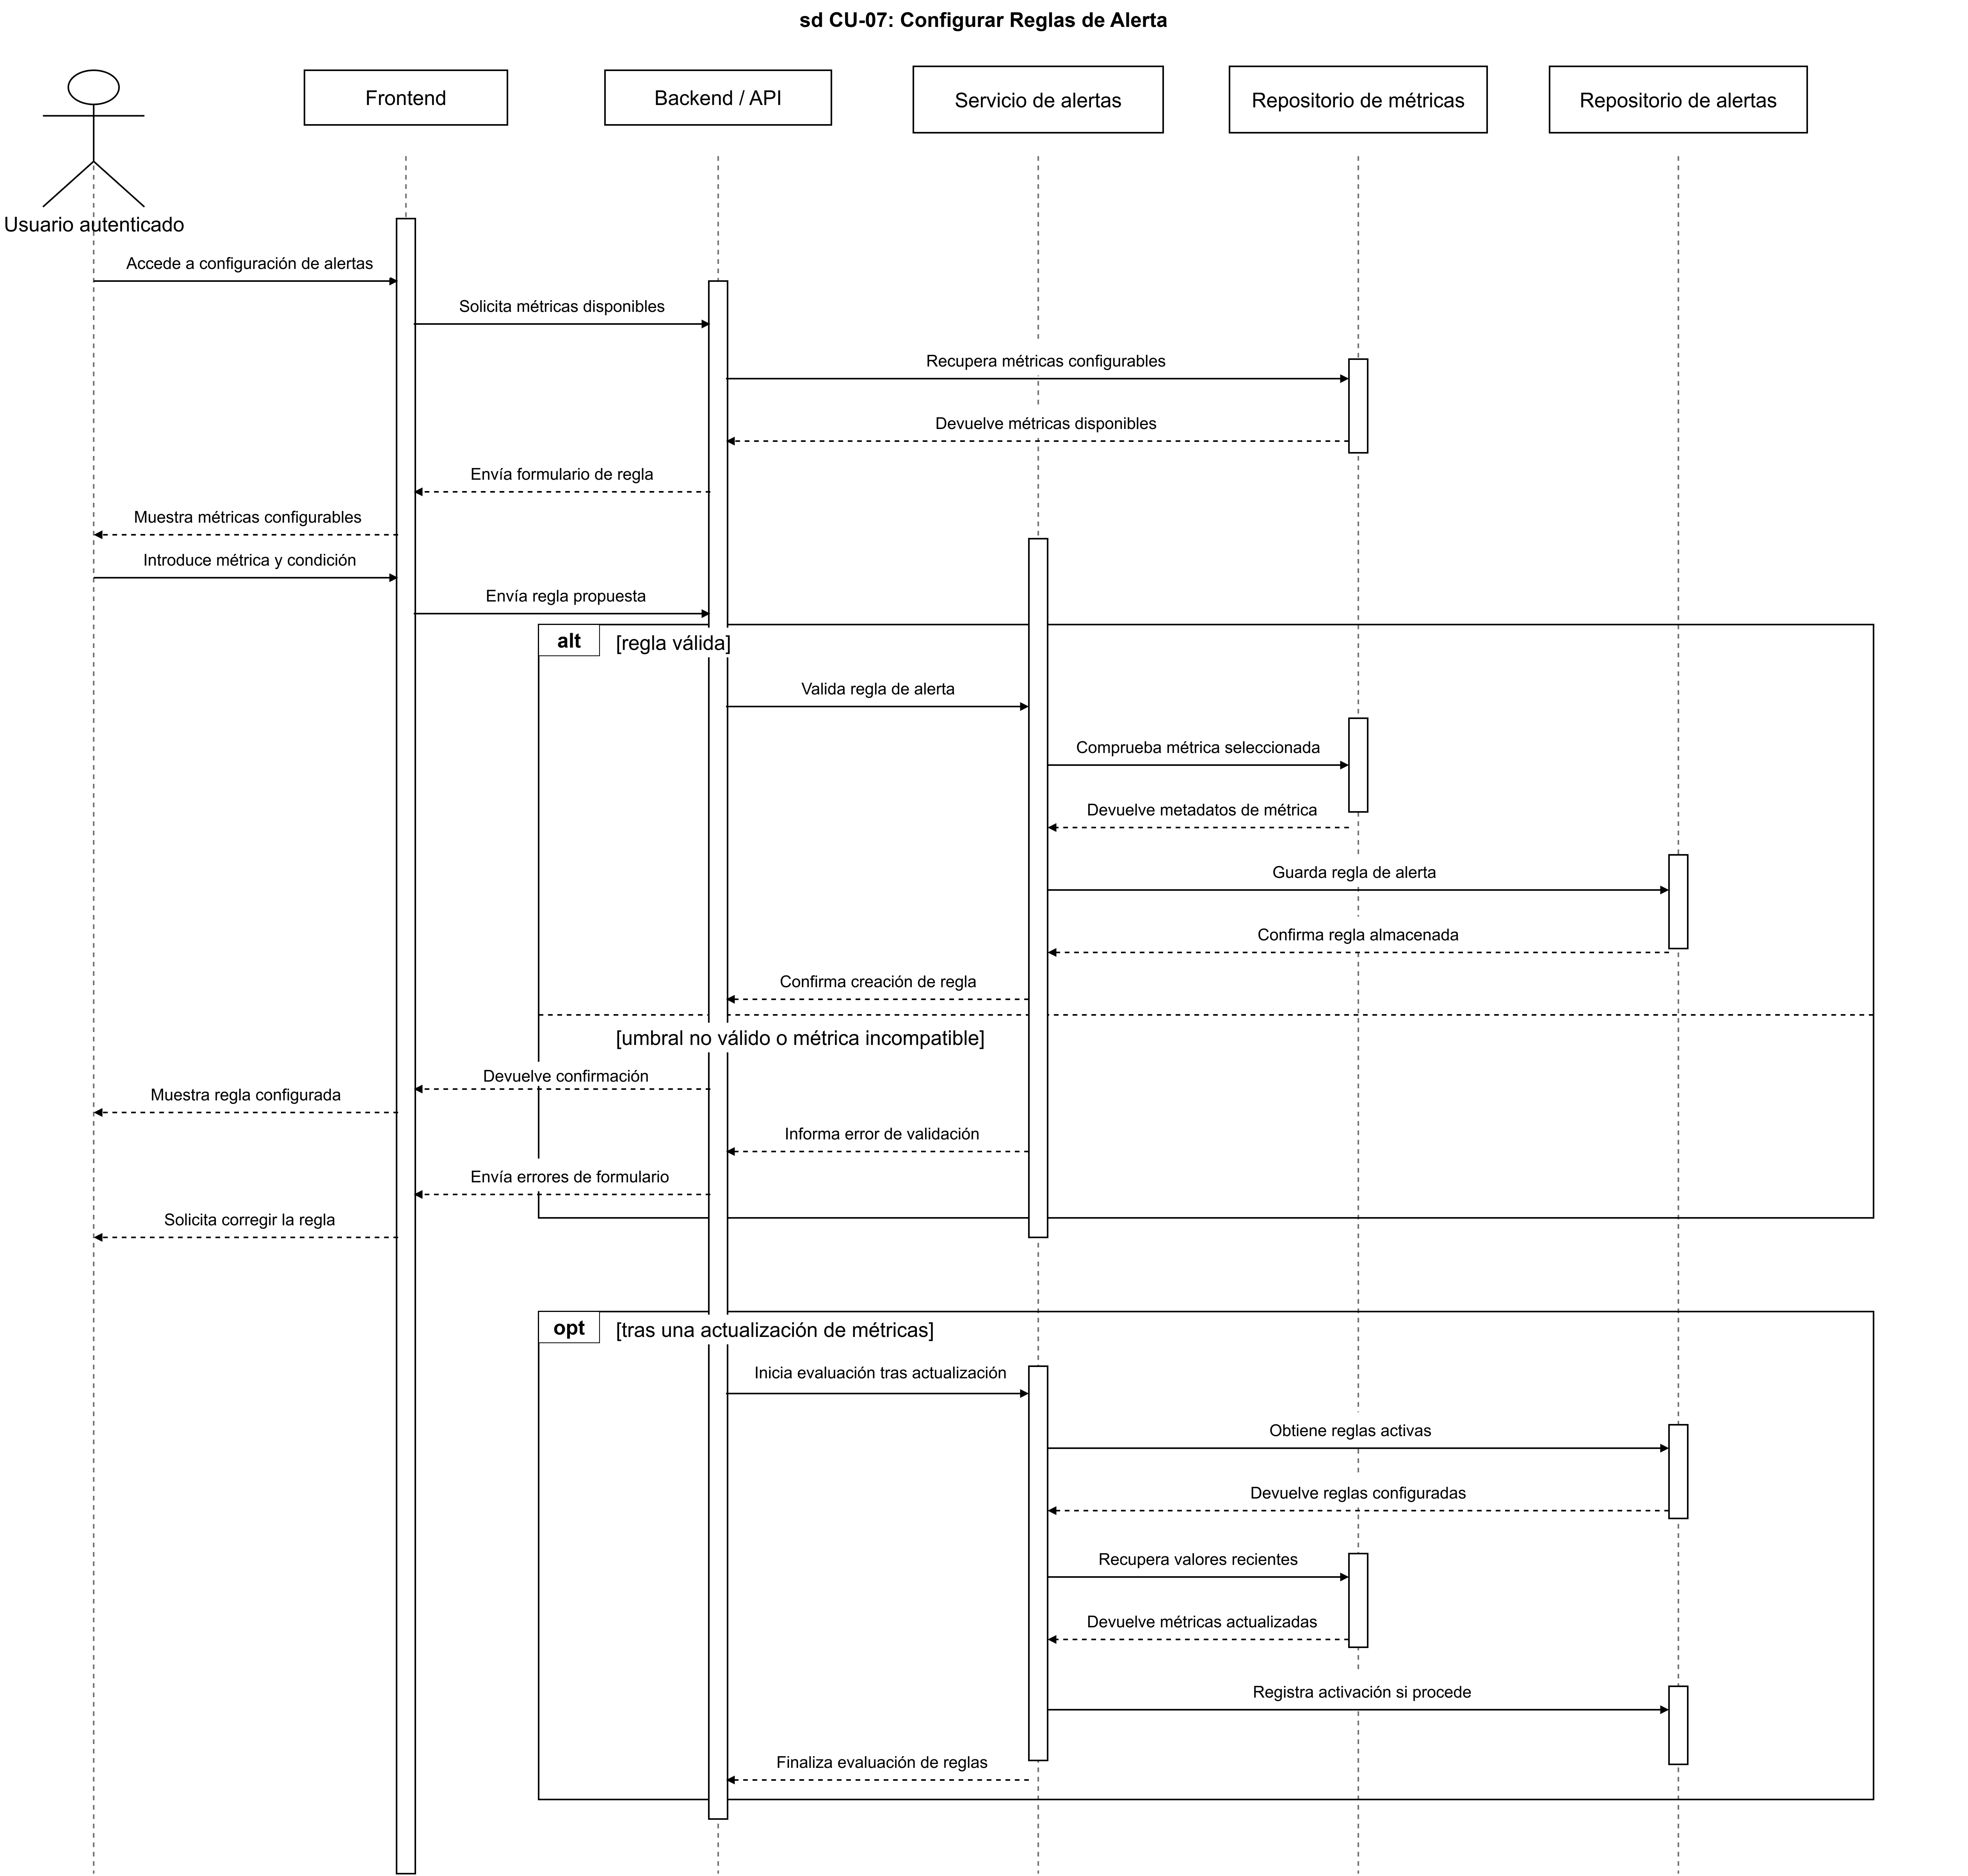
\includegraphics[width=1.08\textwidth]{diagrams/secuencia-cu07-configurar-reglas-alerta.png}}
    \caption{Diagrama de secuencia del caso de uso CU-07}
    \label{fig:secuencia-cu07-configurar-reglas-alerta}
\end{figure}

La Figura~\ref{fig:secuencia-cu07-configurar-reglas-alerta} muestra cómo el usuario autenticado accede a la configuración de alertas, selecciona una métrica y define una condición o umbral. El sistema valida la regla propuesta, comprueba que sea compatible con la métrica seleccionada y la almacena para que pueda evaluarse posteriormente cuando se actualicen las métricas. También se contempla el caso alternativo en el que la regla no es válida o no puede aplicarse a la métrica elegida.
\clearpage
\section{Diagrama de clases}

El diagrama de clases muestra la estructura estática principal del sistema y las relaciones entre los conceptos del dominio. En este caso se representa una vista de análisis previa a la implementación, por lo que las clases describen entidades y responsabilidades del sistema sin depender de una tecnología concreta.

\begin{figure}[htbp]
    \centering
    \makebox[\textwidth][c]{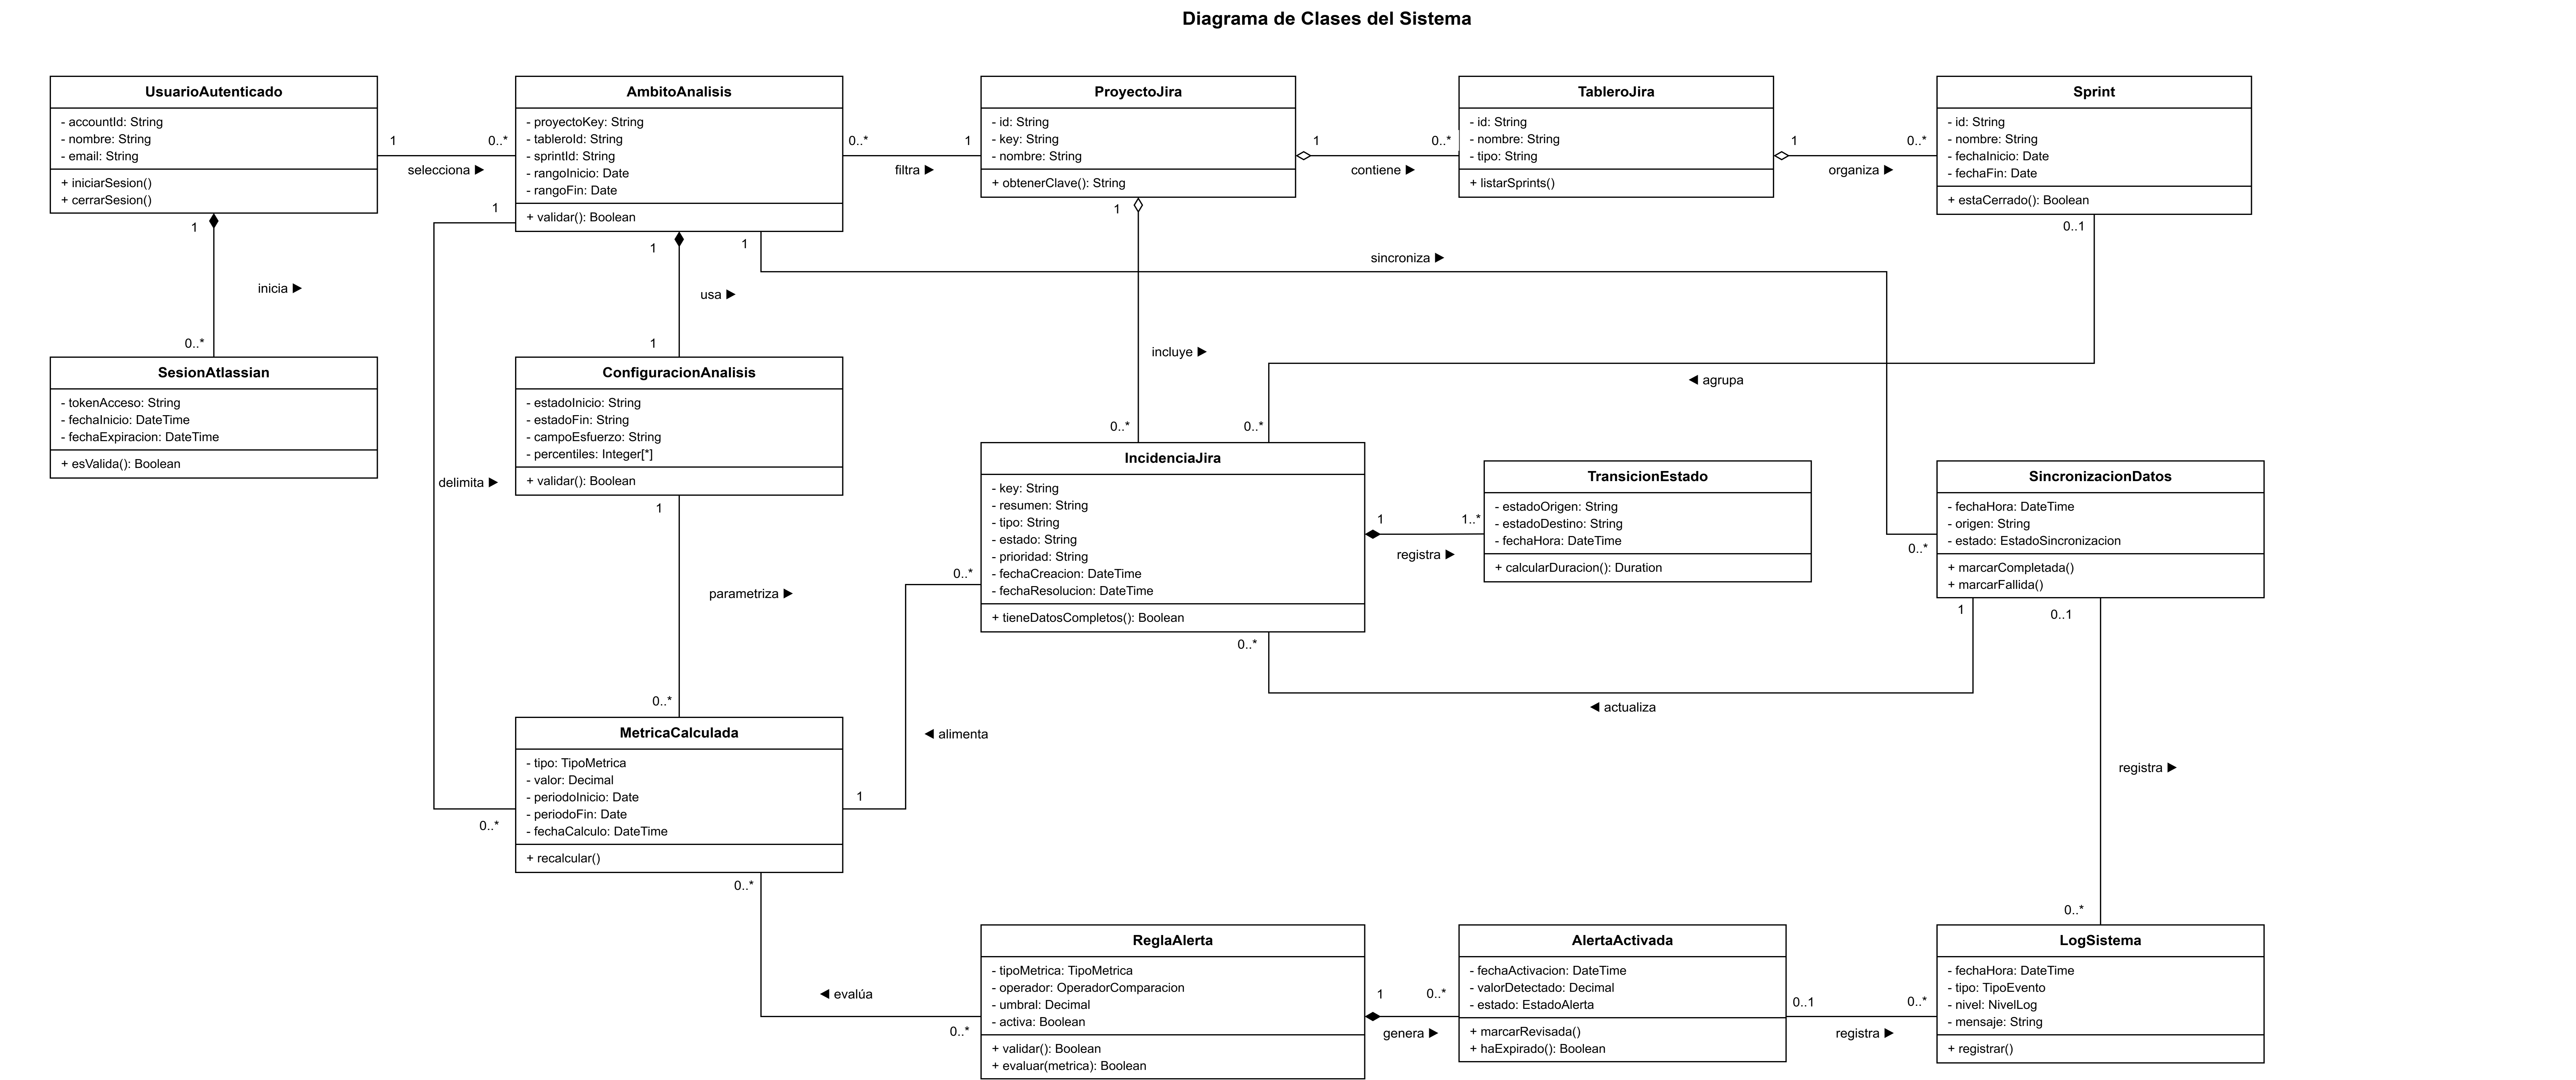
\includegraphics[width=1.25\textwidth]{diagrams/clases-dominio-sistema.png}}
    \caption{Diagrama de clases del sistema}
    \label{fig:clases-dominio-sistema}
\end{figure}

La Figura~\ref{fig:clases-dominio-sistema} se interpreta a partir de los verbos situados sobre cada relación. El triángulo del verbo indica la dirección de lectura y las cardinalidades de los extremos concretan cuántas instancias pueden participar en cada asociación. En cuanto a la notación UML, según la especificación oficial de OMG \cite{OMGUML251}, el rombo blanco representa una agregación, es decir, una relación todo-parte débil en la que la parte puede existir de forma independiente. El rombo negro representa una composición, una relación todo-parte fuerte en la que la parte depende del ciclo de vida del todo. Las clases del diagrama son las siguientes:

\begin{itemize}
    \item \texttt{UsuarioAutenticado}: representa al usuario que accede al sistema. Inicia sesiones de Atlassian y selecciona los ámbitos de análisis sobre los que desea trabajar.
    \item \texttt{SesionAtlassian}: recoge la sesión iniciada mediante Atlassian. Queda asociada al usuario autenticado que la ha creado.
    \item \texttt{AmbitoAnalisis}: define el alcance funcional del análisis. Usa una configuración de análisis, filtra proyectos de Jira, sincroniza datos y delimita las métricas calculadas.
    \item \texttt{ConfiguracionAnalisis}: contiene los criterios de cálculo, filtros y parámetros seleccionados por el usuario. Parametriza las métricas calculadas que se obtienen para un ámbito.
    \item \texttt{ProyectoJira}: representa un proyecto procedente de Jira. Es filtrado por el ámbito de análisis, contiene tableros e incluye incidencias.
    \item \texttt{TableroJira}: modela un tablero de trabajo de Jira. Pertenece a un proyecto y organiza los sprints utilizados en el análisis.
    \item \texttt{Sprint}: representa una iteración de trabajo. Está organizado por un tablero y agrupa las incidencias planificadas o revisadas durante ese periodo.
    \item \texttt{IncidenciaJira}: modela una tarea, historia, error u otro elemento importado desde Jira. Pertenece al proyecto, puede estar agrupada en un sprint, registra transiciones de estado, es actualizada por la sincronización y alimenta el cálculo de métricas.
    \item \texttt{TransicionEstado}: representa un cambio de estado de una incidencia. Queda registrada por la incidencia a la que pertenece y permite analizar tiempos de flujo.
    \item \texttt{SincronizacionDatos}: representa el proceso de actualización de información desde Jira. Se ejecuta dentro de un ámbito de análisis, actualiza incidencias y registra eventos en el log del sistema.
    \item \texttt{MetricaCalculada}: almacena el resultado de aplicar los criterios de análisis. Está parametrizada por la configuración, delimitada por el ámbito y alimentada por las incidencias; además, puede ser evaluada por reglas de alerta.
    \item \texttt{ReglaAlerta}: define una condición o umbral configurable. Evalúa métricas calculadas y genera alertas cuando se cumplen sus condiciones.
    \item \texttt{AlertaActivada}: representa una alerta producida por una regla. Se genera a partir de una regla de alerta y registra su aparición en el log del sistema.
    \item \texttt{LogSistema}: recoge eventos relevantes del sistema. Registra tanto procesos de sincronización como alertas activadas para facilitar la trazabilidad.
\end{itemize}

\clearpage
\section{Diagrama entidad-relación de la base de datos}

El diagrama entidad-relación describe la estructura lógica prevista para la persistencia del sistema. A diferencia del diagrama de clases, que representa conceptos del dominio y responsabilidades de análisis, este modelo se centra en tablas, claves primarias, claves foráneas y cardinalidades. Para facilitar su lectura se emplean entidades rectangulares con sus atributos internos y relaciones representadas mediante rombos, siguiendo la forma habitual de los diagramas entidad-relación y las formas disponibles en draw.io para modelos de bases de datos~\cite{DrawioERTables}. Cada rombo contiene un verbo que describe la relación y las cardinalidades se sitúan junto a los extremos conectados. Los nombres de tablas y columnas se han planteado en minúsculas y con \texttt{snake\_case}, siguiendo criterios habituales de estilo SQL~\cite{HolywellSQLStyle}; además, se evitan estructuras innecesariamente complejas para mantener un diseño comprensible y normalizado, de acuerdo con las recomendaciones generales de diseño relacional recogidas por Karwin~\cite{Karwin2010SQLAntipatterns}.

\begin{figure}[htbp]
    \centering
    \makebox[\textwidth][c]{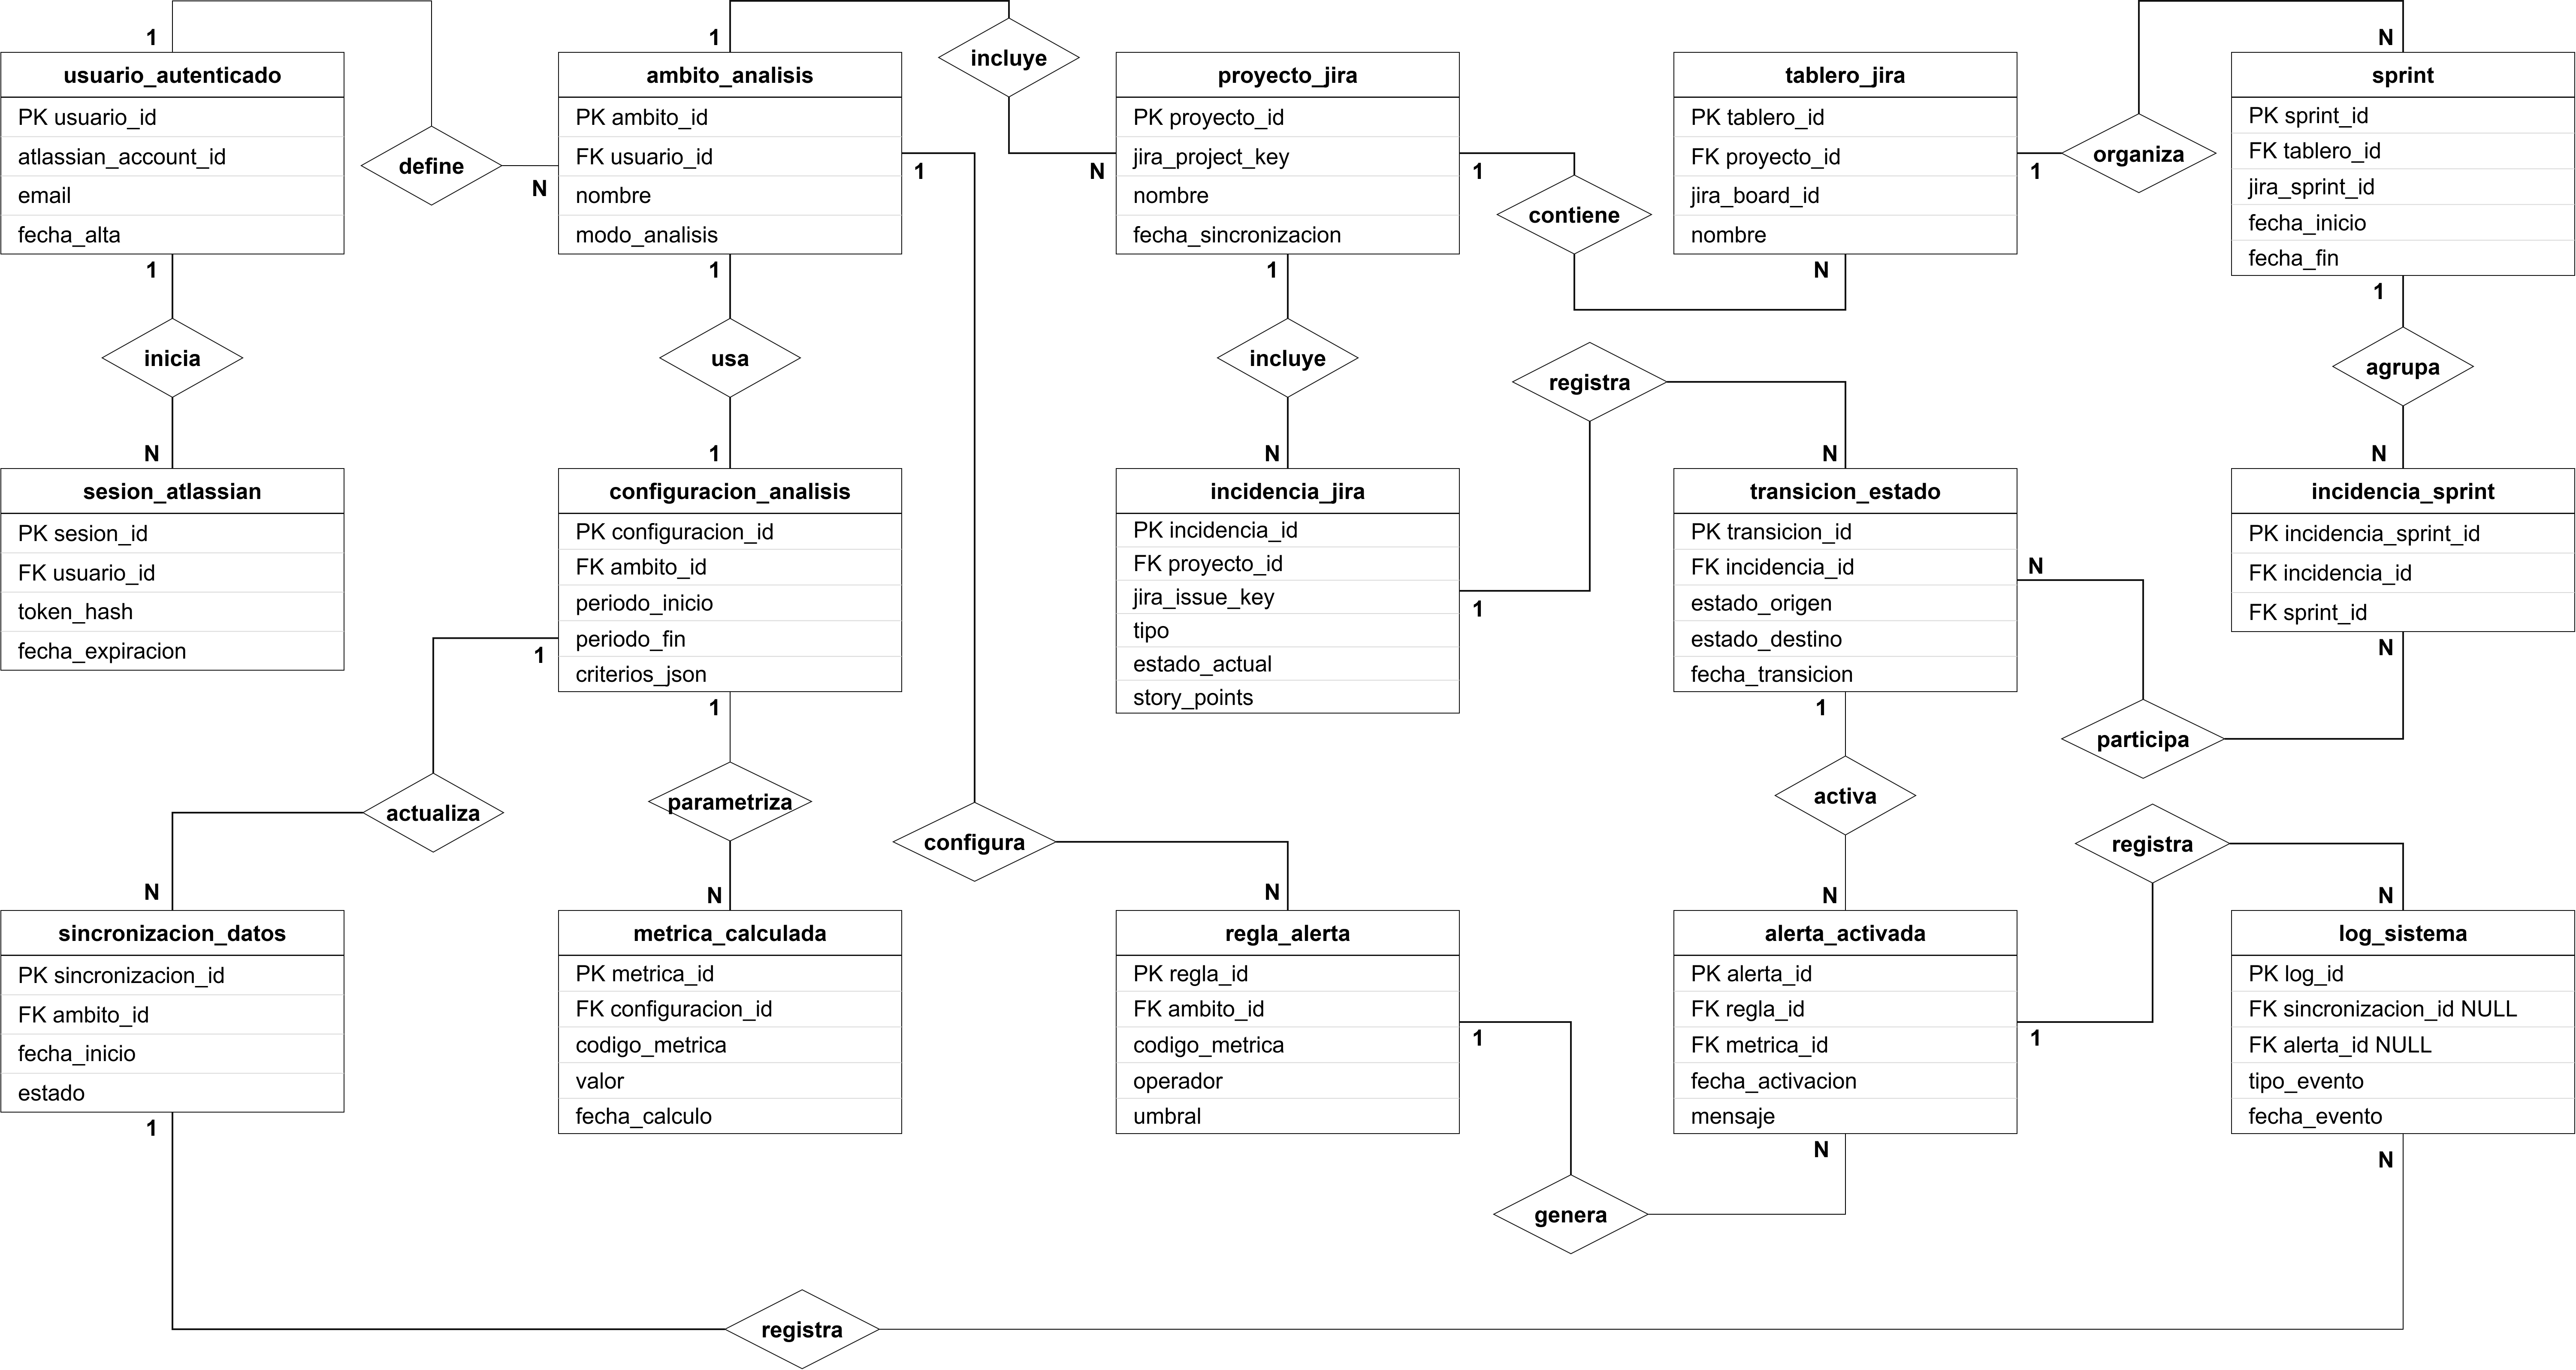
\includegraphics[width=1.25\textwidth]{diagrams/entidad-relacion-base-datos.png}}
    \caption{Diagrama entidad-relación de la base de datos}
    \label{fig:entidad-relacion-base-datos}
\end{figure}

La Figura~\ref{fig:entidad-relacion-base-datos} toma como referencia las entidades principales del diagrama de clases, pero las adapta a un modelo persistente. Las tablas puente \texttt{ambito\_proyecto} e \texttt{incidencia\_sprint} permiten resolver relaciones de muchos a muchos sin duplicar información ni forzar dependencias artificiales.

\begin{itemize}
    \item \texttt{usuario\_autenticado}, \texttt{sesion\_atlassian}, \texttt{ambito\_analisis} y \texttt{configuracion\_analisis}: almacenan la información del usuario, sus sesiones de Atlassian y los criterios de análisis definidos para cada ámbito. Un usuario puede iniciar varias sesiones y definir varios ámbitos; cada ámbito mantiene una configuración de análisis.
    \item \texttt{proyecto\_jira}, \texttt{tablero\_jira}, \texttt{sprint}, \texttt{incidencia\_jira} y \texttt{transicion\_estado}: representan los datos sincronizados desde Jira. Un proyecto puede contener varios tableros e incidencias, un tablero organiza sprints y una incidencia registra sus transiciones de estado para calcular métricas de flujo.
    \item \texttt{ambito\_proyecto} e \texttt{incidencia\_sprint}: actúan como tablas intermedias. La primera asocia ámbitos de análisis con proyectos Jira; la segunda relaciona incidencias con sprints, evitando una relación directa rígida cuando una incidencia pueda aparecer en más de una iteración.
    \item \texttt{sincronizacion\_datos}, \texttt{metrica\_calculada}, \texttt{regla\_alerta}, \texttt{alerta\_activada} y \texttt{log\_sistema}: guardan la actividad interna del sistema. Las sincronizaciones actualizan un ámbito, las métricas se calculan a partir de la configuración vigente, las reglas evalúan dichas métricas y las alertas y logs conservan la trazabilidad del funcionamiento.
\end{itemize}
\clearpage
\section{Diagrama de componentes/arquitectura lógica}

El diagrama de componentes permite representar la organización modular del sistema y las dependencias entre sus partes. Según la especificación oficial de UML de OMG, un componente encapsula una parte sustituible del sistema y expone o requiere interfaces para colaborar con otros elementos~\cite{OMGUML251}. En este trabajo se utiliza esta notación para mostrar una vista lógica de la arquitectura, independiente de decisiones concretas de despliegue.

\begin{figure}[htbp]
    \centering
    \makebox[\textwidth][c]{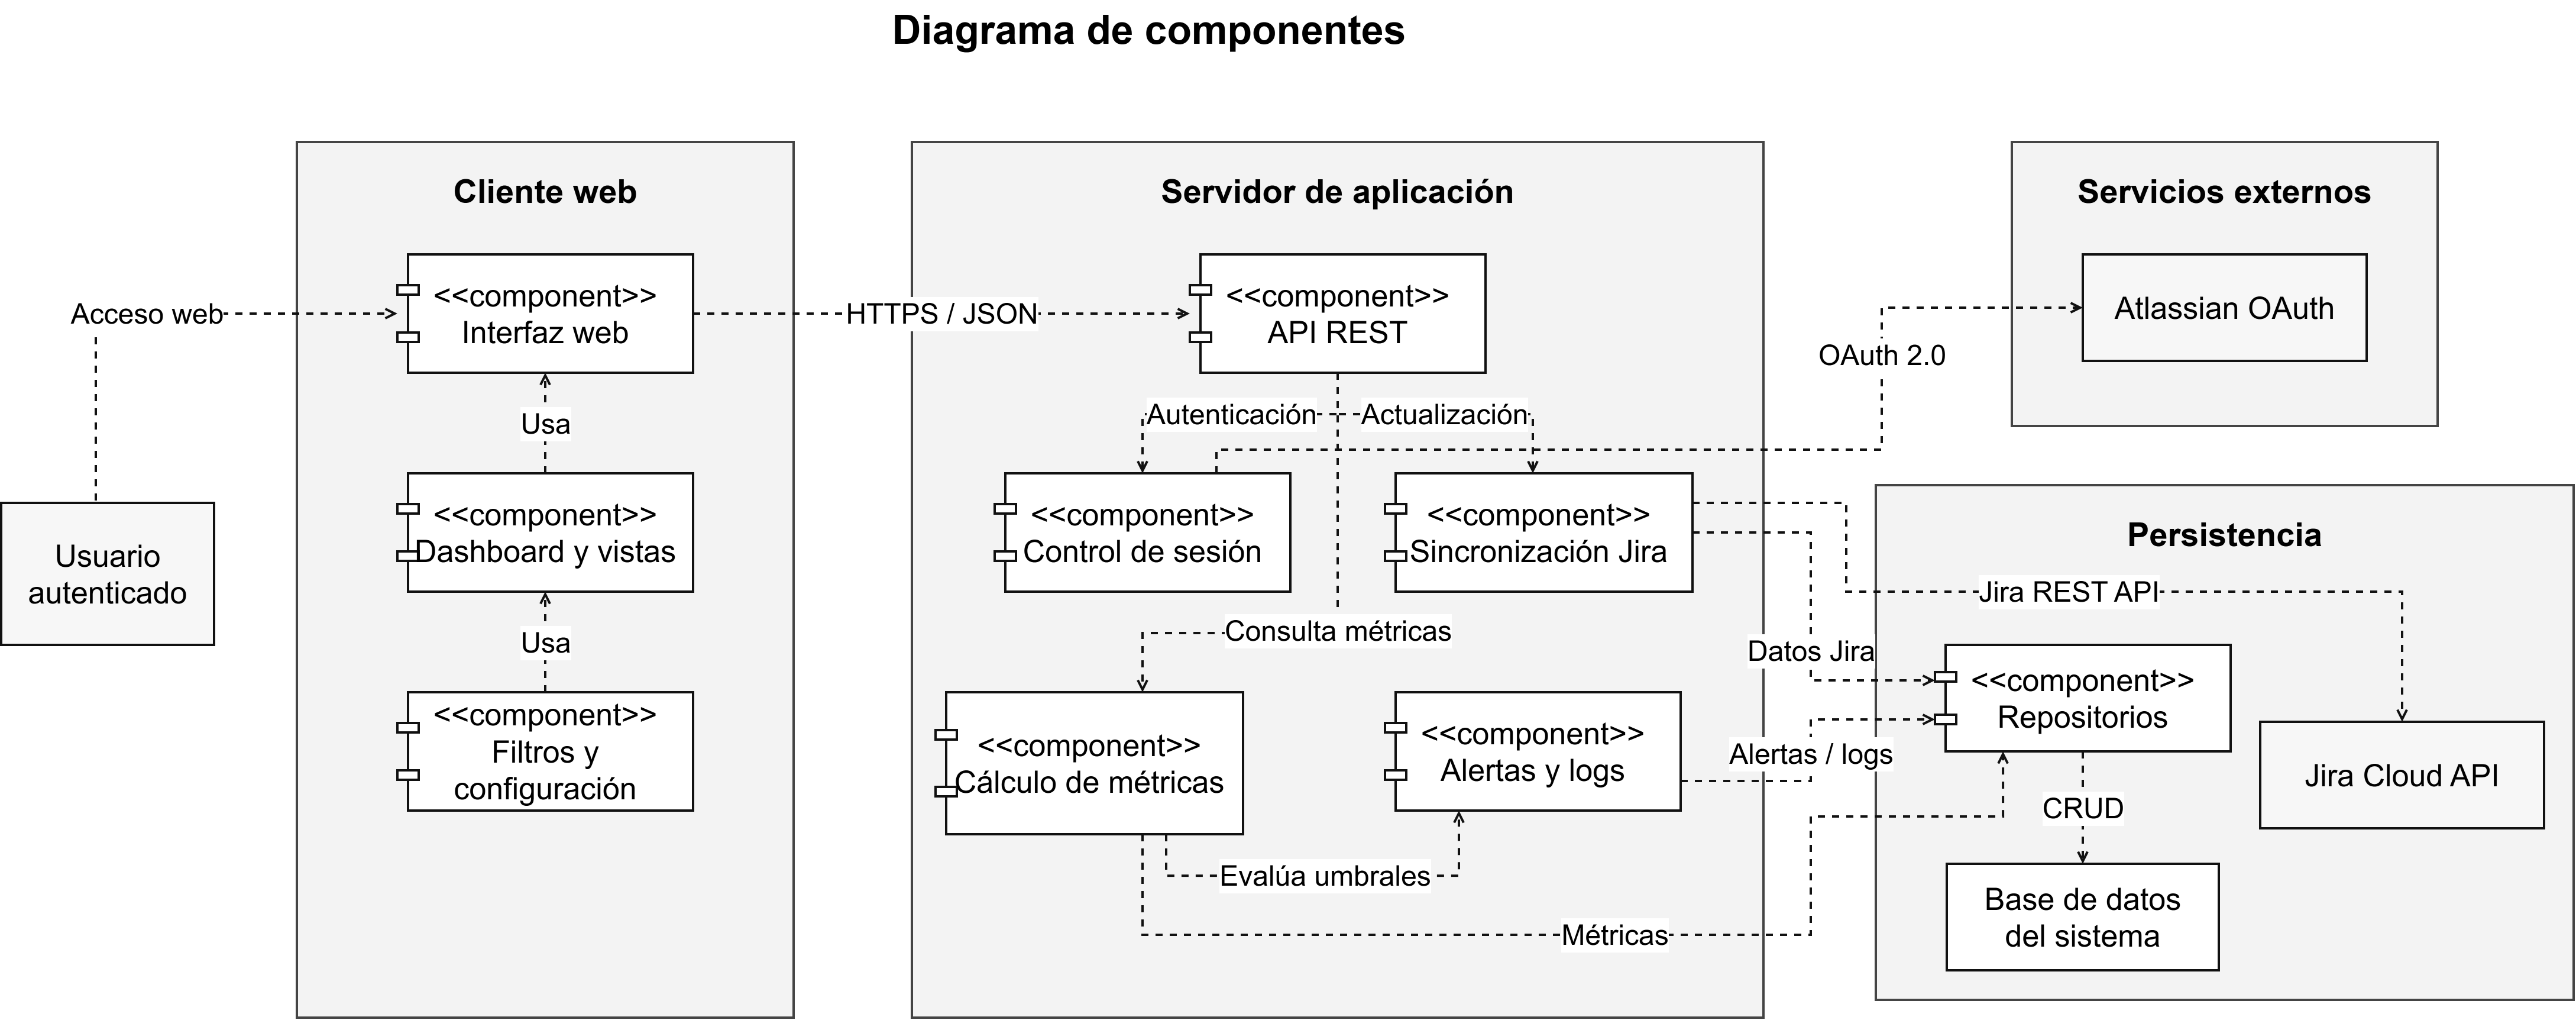
\includegraphics[width=1.25\textwidth]{diagrams/componentes-arquitectura-sistema.png}}
    \caption{Diagrama de componentes y arquitectura lógica del sistema}
    \label{fig:componentes-arquitectura-sistema}
\end{figure}

La Figura~\ref{fig:componentes-arquitectura-sistema} organiza el sistema en cuatro bloques principales: cliente web, servidor de aplicación, servicios externos y persistencia. Las flechas discontinuas representan dependencias entre componentes, es decir, relaciones de uso necesarias para completar las funcionalidades previstas.

\begin{itemize}
    \item \textbf{Cliente web}: agrupa la \texttt{Interfaz web}, el \texttt{Dashboard y vistas} y los componentes de \texttt{Filtros y configuración}. Este bloque permite al usuario autenticado consultar métricas, modificar criterios de análisis y acceder a las vistas principales del sistema.
    \item \textbf{Servidor de aplicación}: contiene la \texttt{API REST}, que centraliza las peticiones del cliente, y los componentes internos encargados del control de sesión, la sincronización con Jira, el cálculo de métricas y la gestión de alertas y logs.
    \item \textbf{Servicios externos}: representan las dependencias con Atlassian. \texttt{Atlassian OAuth} se utiliza para la autenticación del usuario y \texttt{Jira Cloud API} proporciona los datos de proyectos, tableros, sprints e incidencias.
    \item \textbf{Persistencia}: incluye los \texttt{Repositorios}, que aíslan el acceso a datos, y la \texttt{Base de datos del sistema}, donde se almacenan datos sincronizados, configuraciones, métricas calculadas, alertas y logs.
\end{itemize}

Las relaciones principales muestran que el usuario accede al cliente web, el cliente consume la \texttt{API REST} mediante peticiones HTTP y el backend coordina las operaciones internas. El \texttt{Control de sesión} depende de \texttt{Atlassian OAuth}; la \texttt{Sincronización Jira} consulta \texttt{Jira Cloud API}; el \texttt{Cálculo de métricas} trabaja sobre los datos sincronizados; y el componente de \texttt{Alertas y logs} registra eventos y evalúa umbrales a partir de las métricas disponibles. Finalmente, los repositorios concentran la lectura y escritura sobre la base de datos para mantener separada la lógica de negocio del almacenamiento.




